\documentclass[twoside]{book}

% Packages required by doxygen
\usepackage{fixltx2e}
\usepackage{calc}
\usepackage{doxygen}
\usepackage{graphicx}
\usepackage[utf8]{inputenc}
\usepackage{makeidx}
\usepackage{multicol}
\usepackage{multirow}
\PassOptionsToPackage{warn}{textcomp}
\usepackage{textcomp}
\usepackage[nointegrals]{wasysym}
\usepackage[table]{xcolor}

% Font selection
\usepackage[T1]{fontenc}
\usepackage{mathptmx}
\usepackage[scaled=.90]{helvet}
\usepackage{courier}
\usepackage{amssymb}
\usepackage{sectsty}
\renewcommand{\familydefault}{\sfdefault}
\allsectionsfont{%
  \fontseries{bc}\selectfont%
  \color{darkgray}%
}
\renewcommand{\DoxyLabelFont}{%
  \fontseries{bc}\selectfont%
  \color{darkgray}%
}
\newcommand{\+}{\discretionary{\mbox{\scriptsize$\hookleftarrow$}}{}{}}

% Page & text layout
\usepackage{geometry}
\geometry{%
  a4paper,%
  top=2.5cm,%
  bottom=2.5cm,%
  left=2.5cm,%
  right=2.5cm%
}
\tolerance=750
\hfuzz=15pt
\hbadness=750
\setlength{\emergencystretch}{15pt}
\setlength{\parindent}{0cm}
\setlength{\parskip}{0.2cm}
\makeatletter
\renewcommand{\paragraph}{%
  \@startsection{paragraph}{4}{0ex}{-1.0ex}{1.0ex}{%
    \normalfont\normalsize\bfseries\SS@parafont%
  }%
}
\renewcommand{\subparagraph}{%
  \@startsection{subparagraph}{5}{0ex}{-1.0ex}{1.0ex}{%
    \normalfont\normalsize\bfseries\SS@subparafont%
  }%
}
\makeatother

% Headers & footers
\usepackage{fancyhdr}
\pagestyle{fancyplain}
\fancyhead[LE]{\fancyplain{}{\bfseries\thepage}}
\fancyhead[CE]{\fancyplain{}{}}
\fancyhead[RE]{\fancyplain{}{\bfseries\leftmark}}
\fancyhead[LO]{\fancyplain{}{\bfseries\rightmark}}
\fancyhead[CO]{\fancyplain{}{}}
\fancyhead[RO]{\fancyplain{}{\bfseries\thepage}}
\fancyfoot[LE]{\fancyplain{}{}}
\fancyfoot[CE]{\fancyplain{}{}}
\fancyfoot[RE]{\fancyplain{}{\bfseries\scriptsize Generated on Sun Dec 7 2014 23\+:54\+:12 for Search Engine by Doxygen }}
\fancyfoot[LO]{\fancyplain{}{\bfseries\scriptsize Generated on Sun Dec 7 2014 23\+:54\+:12 for Search Engine by Doxygen }}
\fancyfoot[CO]{\fancyplain{}{}}
\fancyfoot[RO]{\fancyplain{}{}}
\renewcommand{\footrulewidth}{0.4pt}
\renewcommand{\chaptermark}[1]{%
  \markboth{#1}{}%
}
\renewcommand{\sectionmark}[1]{%
  \markright{\thesection\ #1}%
}

% Indices & bibliography
\usepackage{natbib}
\usepackage[titles]{tocloft}
\setcounter{tocdepth}{3}
\setcounter{secnumdepth}{5}
\makeindex

% Hyperlinks (required, but should be loaded last)
\usepackage{ifpdf}
\ifpdf
  \usepackage[pdftex,pagebackref=true]{hyperref}
\else
  \usepackage[ps2pdf,pagebackref=true]{hyperref}
\fi
\hypersetup{%
  colorlinks=true,%
  linkcolor=blue,%
  citecolor=blue,%
  unicode%
}

% Custom commands
\newcommand{\clearemptydoublepage}{%
  \newpage{\pagestyle{empty}\cleardoublepage}%
}


%===== C O N T E N T S =====

\begin{document}

% Titlepage & ToC
\hypersetup{pageanchor=false,
             bookmarks=true,
             bookmarksnumbered=true,
             pdfencoding=unicode
            }
\pagenumbering{roman}
\begin{titlepage}
\vspace*{7cm}
\begin{center}%
{\Large Search Engine \\[1ex]\large v1.\+0 }\\
\vspace*{1cm}
{\large Generated by Doxygen 1.8.8}\\
\vspace*{0.5cm}
{\small Sun Dec 7 2014 23:54:12}\\
\end{center}
\end{titlepage}
\clearemptydoublepage
\tableofcontents
\clearemptydoublepage
\pagenumbering{arabic}
\hypersetup{pageanchor=true}

%--- Begin generated contents ---
\chapter{Hierarchical Index}
\section{Class Hierarchy}
This inheritance list is sorted roughly, but not completely, alphabetically\+:\begin{DoxyCompactList}
\item \contentsline{section}{rapidxml\+:\+:attribute\+\_\+iterator$<$ Ch $>$}{\pageref{classrapidxml_1_1attribute__iterator}}{}
\item \contentsline{section}{A\+V\+L\+Tree$<$ T $>$}{\pageref{class_a_v_l_tree}}{}
\item \contentsline{section}{A\+V\+L\+Tree$<$ std\+:\+:string $>$}{\pageref{class_a_v_l_tree}}{}
\item \contentsline{section}{A\+V\+L\+Tree$<$ unique\+Words $>$}{\pageref{class_a_v_l_tree}}{}
\item \contentsline{section}{A\+V\+L\+Tree$<$ Word\+Info $>$}{\pageref{class_a_v_l_tree}}{}
\item exception\begin{DoxyCompactList}
\item \contentsline{section}{rapidxml\+:\+:parse\+\_\+error}{\pageref{classrapidxml_1_1parse__error}}{}
\end{DoxyCompactList}
\item \contentsline{section}{rapidxml\+:\+:file$<$ Ch $>$}{\pageref{classrapidxml_1_1file}}{}
\item \contentsline{section}{Index\+Driver}{\pageref{class_index_driver}}{}
\item \contentsline{section}{rapidxml\+:\+:memory\+\_\+pool$<$ Ch $>$}{\pageref{classrapidxml_1_1memory__pool}}{}
\begin{DoxyCompactList}
\item \contentsline{section}{rapidxml\+:\+:xml\+\_\+document$<$ Ch $>$}{\pageref{singletonrapidxml_1_1xml__document}}{}
\end{DoxyCompactList}
\item \contentsline{section}{rapidxml\+:\+:node\+\_\+iterator$<$ Ch $>$}{\pageref{classrapidxml_1_1node__iterator}}{}
\item \contentsline{section}{Query\+Processor}{\pageref{class_query_processor}}{}
\item \contentsline{section}{stop\+Worder}{\pageref{classstop_worder}}{}
\item \contentsline{section}{unique\+Words}{\pageref{classunique_words}}{}
\item \contentsline{section}{Virtual\+Indexer}{\pageref{class_virtual_indexer}}{}
\begin{DoxyCompactList}
\item \contentsline{section}{A\+V\+L\+Indexer}{\pageref{class_a_v_l_indexer}}{}
\end{DoxyCompactList}
\item \contentsline{section}{Word\+Info}{\pageref{class_word_info}}{}
\item \contentsline{section}{rapidxml\+:\+:xml\+\_\+base$<$ Ch $>$}{\pageref{classrapidxml_1_1xml__base}}{}
\begin{DoxyCompactList}
\item \contentsline{section}{rapidxml\+:\+:xml\+\_\+attribute$<$ Ch $>$}{\pageref{singletonrapidxml_1_1xml__attribute}}{}
\item \contentsline{section}{rapidxml\+:\+:xml\+\_\+node$<$ Ch $>$}{\pageref{singletonrapidxml_1_1xml__node}}{}
\begin{DoxyCompactList}
\item \contentsline{section}{rapidxml\+:\+:xml\+\_\+document$<$ Ch $>$}{\pageref{singletonrapidxml_1_1xml__document}}{}
\end{DoxyCompactList}
\end{DoxyCompactList}
\item \contentsline{section}{X\+M\+L\+Parser}{\pageref{class_x_m_l_parser}}{}
\item \contentsline{section}{X\+M\+L\+Passer}{\pageref{class_x_m_l_passer}}{}
\end{DoxyCompactList}

\chapter{Class Index}
\section{Class List}
Here are the classes, structs, unions and interfaces with brief descriptions\+:\begin{DoxyCompactList}
\item\contentsline{section}{\hyperlink{classrapidxml_1_1attribute__iterator}{rapidxml\+::attribute\+\_\+iterator$<$ Ch $>$} \\*Iterator of child attributes of \hyperlink{singletonrapidxml_1_1xml__node}{xml\+\_\+node} }{\pageref{classrapidxml_1_1attribute__iterator}}{}
\item\contentsline{section}{\hyperlink{class_a_v_l_indexer}{A\+V\+L\+Indexer} }{\pageref{class_a_v_l_indexer}}{}
\item\contentsline{section}{\hyperlink{class_a_v_l_tree}{A\+V\+L\+Tree$<$ T $>$} }{\pageref{class_a_v_l_tree}}{}
\item\contentsline{section}{\hyperlink{classrapidxml_1_1file}{rapidxml\+::file$<$ Ch $>$} \\*Represents data loaded from a file }{\pageref{classrapidxml_1_1file}}{}
\item\contentsline{section}{\hyperlink{class_index_driver}{Index\+Driver} }{\pageref{class_index_driver}}{}
\item\contentsline{section}{\hyperlink{classrapidxml_1_1memory__pool}{rapidxml\+::memory\+\_\+pool$<$ Ch $>$} }{\pageref{classrapidxml_1_1memory__pool}}{}
\item\contentsline{section}{\hyperlink{classrapidxml_1_1node__iterator}{rapidxml\+::node\+\_\+iterator$<$ Ch $>$} \\*Iterator of child nodes of \hyperlink{singletonrapidxml_1_1xml__node}{xml\+\_\+node} }{\pageref{classrapidxml_1_1node__iterator}}{}
\item\contentsline{section}{\hyperlink{classrapidxml_1_1parse__error}{rapidxml\+::parse\+\_\+error} }{\pageref{classrapidxml_1_1parse__error}}{}
\item\contentsline{section}{\hyperlink{class_query_processor}{Query\+Processor} }{\pageref{class_query_processor}}{}
\item\contentsline{section}{\hyperlink{classstop_worder}{stop\+Worder} }{\pageref{classstop_worder}}{}
\item\contentsline{section}{\hyperlink{classunique_words}{unique\+Words} }{\pageref{classunique_words}}{}
\item\contentsline{section}{\hyperlink{class_virtual_indexer}{Virtual\+Indexer} }{\pageref{class_virtual_indexer}}{}
\item\contentsline{section}{\hyperlink{class_word_info}{Word\+Info} }{\pageref{class_word_info}}{}
\item\contentsline{section}{\hyperlink{singletonrapidxml_1_1xml__attribute}{rapidxml\+::xml\+\_\+attribute$<$ Ch $>$} }{\pageref{singletonrapidxml_1_1xml__attribute}}{}
\item\contentsline{section}{\hyperlink{classrapidxml_1_1xml__base}{rapidxml\+::xml\+\_\+base$<$ Ch $>$} }{\pageref{classrapidxml_1_1xml__base}}{}
\item\contentsline{section}{\hyperlink{singletonrapidxml_1_1xml__document}{rapidxml\+::xml\+\_\+document$<$ Ch $>$} }{\pageref{singletonrapidxml_1_1xml__document}}{}
\item\contentsline{section}{\hyperlink{singletonrapidxml_1_1xml__node}{rapidxml\+::xml\+\_\+node$<$ Ch $>$} }{\pageref{singletonrapidxml_1_1xml__node}}{}
\item\contentsline{section}{\hyperlink{class_x_m_l_parser}{X\+M\+L\+Parser} }{\pageref{class_x_m_l_parser}}{}
\item\contentsline{section}{\hyperlink{class_x_m_l_passer}{X\+M\+L\+Passer} }{\pageref{class_x_m_l_passer}}{}
\end{DoxyCompactList}

\chapter{File Index}
\section{File List}
Here is a list of all documented files with brief descriptions\+:\begin{DoxyCompactList}
\item\contentsline{section}{{\bfseries A\+V\+L\+Indexer.\+h} }{\pageref{_a_v_l_indexer_8h}}{}
\item\contentsline{section}{{\bfseries A\+V\+L\+Tree.\+hpp} }{\pageref{_a_v_l_tree_8hpp}}{}
\item\contentsline{section}{{\bfseries Index\+Driver.\+h} }{\pageref{_index_driver_8h}}{}
\item\contentsline{section}{{\bfseries Query\+Processor.\+h} }{\pageref{_query_processor_8h}}{}
\item\contentsline{section}{\hyperlink{rapidxml_8hpp}{rapidxml.\+hpp} \\*This file contains rapidxml parser and D\+O\+M implementation }{\pageref{rapidxml_8hpp}}{}
\item\contentsline{section}{\hyperlink{rapidxml__iterators_8hpp}{rapidxml\+\_\+iterators.\+hpp} \\*This file contains rapidxml iterators }{\pageref{rapidxml__iterators_8hpp}}{}
\item\contentsline{section}{\hyperlink{rapidxml__print_8hpp}{rapidxml\+\_\+print.\+hpp} \\*This file contains rapidxml printer implementation }{\pageref{rapidxml__print_8hpp}}{}
\item\contentsline{section}{\hyperlink{rapidxml__utils_8hpp}{rapidxml\+\_\+utils.\+hpp} }{\pageref{rapidxml__utils_8hpp}}{}
\item\contentsline{section}{{\bfseries Stem.\+h} }{\pageref{_stem_8h}}{}
\item\contentsline{section}{{\bfseries Stop\+Worder.\+h} }{\pageref{_stop_worder_8h}}{}
\item\contentsline{section}{{\bfseries unique\+Words.\+h} }{\pageref{unique_words_8h}}{}
\item\contentsline{section}{{\bfseries Virtual\+Indexer.\+h} }{\pageref{_virtual_indexer_8h}}{}
\item\contentsline{section}{{\bfseries Word\+Info.\+h} }{\pageref{_word_info_8h}}{}
\item\contentsline{section}{{\bfseries X\+M\+Lparser.\+h} }{\pageref{_x_m_lparser_8h}}{}
\item\contentsline{section}{{\bfseries X\+M\+L\+Passer.\+h} }{\pageref{_x_m_l_passer_8h}}{}
\end{DoxyCompactList}

\chapter{Class Documentation}
\hypertarget{classrapidxml_1_1attribute__iterator}{\section{rapidxml\+:\+:attribute\+\_\+iterator$<$ Ch $>$ Class Template Reference}
\label{classrapidxml_1_1attribute__iterator}\index{rapidxml\+::attribute\+\_\+iterator$<$ Ch $>$@{rapidxml\+::attribute\+\_\+iterator$<$ Ch $>$}}
}


Iterator of child attributes of \hyperlink{singletonrapidxml_1_1xml__node}{xml\+\_\+node}.  




{\ttfamily \#include $<$rapidxml\+\_\+iterators.\+hpp$>$}

\subsection*{Public Types}
\begin{DoxyCompactItemize}
\item 
\hypertarget{classrapidxml_1_1attribute__iterator_ad4280d358828ad9c3eb1a787decb162e}{typedef \hyperlink{singletonrapidxml_1_1xml__attribute}{xml\+\_\+attribute}$<$ Ch $>$ {\bfseries value\+\_\+type}}\label{classrapidxml_1_1attribute__iterator_ad4280d358828ad9c3eb1a787decb162e}

\item 
\hypertarget{classrapidxml_1_1attribute__iterator_a097343e44557de14de86b470d3f917d9}{typedef \hyperlink{singletonrapidxml_1_1xml__attribute}{xml\+\_\+attribute}$<$ Ch $>$ \& {\bfseries reference}}\label{classrapidxml_1_1attribute__iterator_a097343e44557de14de86b470d3f917d9}

\item 
\hypertarget{classrapidxml_1_1attribute__iterator_a69acc2e60270d6a062c03c9cb1cf2aa7}{typedef \hyperlink{singletonrapidxml_1_1xml__attribute}{xml\+\_\+attribute}$<$ Ch $>$ $\ast$ {\bfseries pointer}}\label{classrapidxml_1_1attribute__iterator_a69acc2e60270d6a062c03c9cb1cf2aa7}

\item 
\hypertarget{classrapidxml_1_1attribute__iterator_accfd6d8527d32b427496b42f71a2e37a}{typedef std\+::ptrdiff\+\_\+t {\bfseries difference\+\_\+type}}\label{classrapidxml_1_1attribute__iterator_accfd6d8527d32b427496b42f71a2e37a}

\item 
\hypertarget{classrapidxml_1_1attribute__iterator_a97ac5d8b98f5b03c68cc566f5ac0a9e0}{typedef \\*
std\+::bidirectional\+\_\+iterator\+\_\+tag {\bfseries iterator\+\_\+category}}\label{classrapidxml_1_1attribute__iterator_a97ac5d8b98f5b03c68cc566f5ac0a9e0}

\end{DoxyCompactItemize}
\subsection*{Public Member Functions}
\begin{DoxyCompactItemize}
\item 
\hypertarget{classrapidxml_1_1attribute__iterator_a1109344dead88533ae4dd68cea5d9613}{{\bfseries attribute\+\_\+iterator} (\hyperlink{singletonrapidxml_1_1xml__node}{xml\+\_\+node}$<$ Ch $>$ $\ast$node)}\label{classrapidxml_1_1attribute__iterator_a1109344dead88533ae4dd68cea5d9613}

\item 
\hypertarget{classrapidxml_1_1attribute__iterator_a5d8616bdd2d41119e2f342d77b4f56f9}{\hyperlink{singletonrapidxml_1_1xml__attribute}{reference} {\bfseries operator$\ast$} () const }\label{classrapidxml_1_1attribute__iterator_a5d8616bdd2d41119e2f342d77b4f56f9}

\item 
\hypertarget{classrapidxml_1_1attribute__iterator_a0975adffe3d178c0ac83652b9ab78791}{\hyperlink{singletonrapidxml_1_1xml__attribute}{pointer} {\bfseries operator-\/$>$} () const }\label{classrapidxml_1_1attribute__iterator_a0975adffe3d178c0ac83652b9ab78791}

\item 
\hypertarget{classrapidxml_1_1attribute__iterator_afe7d15a4a1b228f97f1d4ebd4f3f6cca}{\hyperlink{classrapidxml_1_1attribute__iterator}{attribute\+\_\+iterator} \& {\bfseries operator++} ()}\label{classrapidxml_1_1attribute__iterator_afe7d15a4a1b228f97f1d4ebd4f3f6cca}

\item 
\hypertarget{classrapidxml_1_1attribute__iterator_a82c8859b9eebd45caa3afc25b9e78c36}{\hyperlink{classrapidxml_1_1attribute__iterator}{attribute\+\_\+iterator} {\bfseries operator++} (int)}\label{classrapidxml_1_1attribute__iterator_a82c8859b9eebd45caa3afc25b9e78c36}

\item 
\hypertarget{classrapidxml_1_1attribute__iterator_af22f1ad3c11d3269b43b49e29b89d7d1}{\hyperlink{classrapidxml_1_1attribute__iterator}{attribute\+\_\+iterator} \& {\bfseries operator-\/-\/} ()}\label{classrapidxml_1_1attribute__iterator_af22f1ad3c11d3269b43b49e29b89d7d1}

\item 
\hypertarget{classrapidxml_1_1attribute__iterator_af52a8562ab1b2c0391cdde79f55e4a6f}{\hyperlink{classrapidxml_1_1attribute__iterator}{attribute\+\_\+iterator} {\bfseries operator-\/-\/} (int)}\label{classrapidxml_1_1attribute__iterator_af52a8562ab1b2c0391cdde79f55e4a6f}

\item 
\hypertarget{classrapidxml_1_1attribute__iterator_ab1dc8dd11d21e145a4e3f76d46aead0d}{bool {\bfseries operator==} (const \hyperlink{classrapidxml_1_1attribute__iterator}{attribute\+\_\+iterator}$<$ Ch $>$ \&rhs)}\label{classrapidxml_1_1attribute__iterator_ab1dc8dd11d21e145a4e3f76d46aead0d}

\item 
\hypertarget{classrapidxml_1_1attribute__iterator_a39e8cf336c324521fd9c720abf280d88}{bool {\bfseries operator!=} (const \hyperlink{classrapidxml_1_1attribute__iterator}{attribute\+\_\+iterator}$<$ Ch $>$ \&rhs)}\label{classrapidxml_1_1attribute__iterator_a39e8cf336c324521fd9c720abf280d88}

\end{DoxyCompactItemize}


\subsection{Detailed Description}
\subsubsection*{template$<$class Ch$>$class rapidxml\+::attribute\+\_\+iterator$<$ Ch $>$}

Iterator of child attributes of \hyperlink{singletonrapidxml_1_1xml__node}{xml\+\_\+node}. 

The documentation for this class was generated from the following file\+:\begin{DoxyCompactItemize}
\item 
\hyperlink{rapidxml__iterators_8hpp}{rapidxml\+\_\+iterators.\+hpp}\end{DoxyCompactItemize}

\hypertarget{class_a_v_l_indexer}{\section{A\+V\+L\+Indexer Class Reference}
\label{class_a_v_l_indexer}\index{A\+V\+L\+Indexer@{A\+V\+L\+Indexer}}
}
Inheritance diagram for A\+V\+L\+Indexer\+:\begin{figure}[H]
\begin{center}
\leavevmode
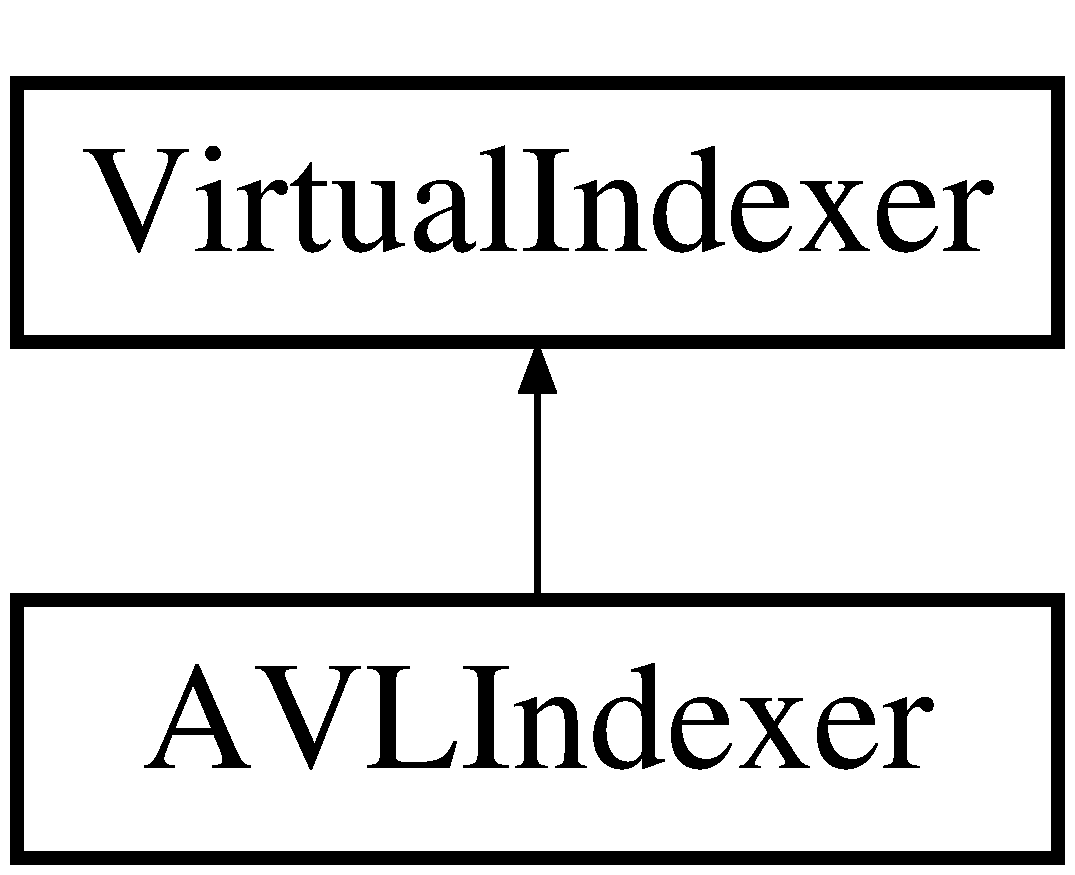
\includegraphics[height=2.000000cm]{class_a_v_l_indexer}
\end{center}
\end{figure}
\subsection*{Public Member Functions}
\begin{DoxyCompactItemize}
\item 
\hypertarget{class_a_v_l_indexer_a23e1a552dec97821bc8090795513b513}{virtual void {\bfseries insert} (string word, string S\+H\+A1id, int frequency, int page\+Num)}\label{class_a_v_l_indexer_a23e1a552dec97821bc8090795513b513}

\item 
\hypertarget{class_a_v_l_indexer_a1c5073ebd52743d66ae2ae4a7376945a}{virtual \hyperlink{class_a_v_l_tree}{A\+V\+L\+Tree}$<$ \hyperlink{class_word_info}{Word\+Info} $>$ {\bfseries search} (string word)}\label{class_a_v_l_indexer_a1c5073ebd52743d66ae2ae4a7376945a}

\item 
\hypertarget{class_a_v_l_indexer_a86efca0a4e959fa4ea41e7b444edc1b1}{virtual void {\bfseries delete\+Index} ()}\label{class_a_v_l_indexer_a86efca0a4e959fa4ea41e7b444edc1b1}

\item 
\hypertarget{class_a_v_l_indexer_a7bfb4ec1c8b17045ce5d950747d318e0}{virtual void {\bfseries save\+Index} ()}\label{class_a_v_l_indexer_a7bfb4ec1c8b17045ce5d950747d318e0}

\item 
\hypertarget{class_a_v_l_indexer_aa578ab6696c640480beee1f905cfea60}{virtual void {\bfseries print\+Index} (ostream \&ostrm)}\label{class_a_v_l_indexer_aa578ab6696c640480beee1f905cfea60}

\item 
\hypertarget{class_a_v_l_indexer_adc22599101f713d2d72d09a8cfdb8253}{virtual bool {\bfseries is\+Found} (string word)}\label{class_a_v_l_indexer_adc22599101f713d2d72d09a8cfdb8253}

\item 
\hypertarget{class_a_v_l_indexer_abe949f9056e016f07094dce1846b90e4}{virtual void {\bfseries increment\+Frequency} (string word, string S\+H\+A1, int freq)}\label{class_a_v_l_indexer_abe949f9056e016f07094dce1846b90e4}

\end{DoxyCompactItemize}


The documentation for this class was generated from the following files\+:\begin{DoxyCompactItemize}
\item 
A\+V\+L\+Indexer.\+h\item 
A\+V\+L\+Indexer.\+cpp\end{DoxyCompactItemize}

\hypertarget{class_a_v_l_tree}{\section{A\+V\+L\+Tree$<$ T $>$ Class Template Reference}
\label{class_a_v_l_tree}\index{A\+V\+L\+Tree$<$ T $>$@{A\+V\+L\+Tree$<$ T $>$}}
}
\subsection*{Public Member Functions}
\begin{DoxyCompactItemize}
\item 
\hypertarget{class_a_v_l_tree_a661fdb05fd0bc8157be56ea729574c38}{{\bfseries A\+V\+L\+Tree} (const \hyperlink{class_a_v_l_tree}{A\+V\+L\+Tree} \&rhs)}\label{class_a_v_l_tree_a661fdb05fd0bc8157be56ea729574c38}

\item 
\hypertarget{class_a_v_l_tree_adf815f7c7638434224d13cd3845dbab0}{bool {\bfseries is\+Found} (const T \&x)}\label{class_a_v_l_tree_adf815f7c7638434224d13cd3845dbab0}

\item 
\hypertarget{class_a_v_l_tree_a078448aa96485249b15fdee43a504ee4}{bool {\bfseries is\+Empty} () const }\label{class_a_v_l_tree_a078448aa96485249b15fdee43a504ee4}

\item 
\hypertarget{class_a_v_l_tree_ab7062b17bcc409f0b9200671482fad01}{void {\bfseries make\+Empty} ()}\label{class_a_v_l_tree_ab7062b17bcc409f0b9200671482fad01}

\item 
\hypertarget{class_a_v_l_tree_aa8f3199f54f1e2a4d9ae0ac16be2344b}{void {\bfseries insert} (const T \&x)}\label{class_a_v_l_tree_aa8f3199f54f1e2a4d9ae0ac16be2344b}

\item 
\hypertarget{class_a_v_l_tree_a5e64e3b797903ffd4d5b8bc4b0adb2f4}{T \& {\bfseries find} (const T \&x)}\label{class_a_v_l_tree_a5e64e3b797903ffd4d5b8bc4b0adb2f4}

\item 
\hypertarget{class_a_v_l_tree_a6591eaa28e62eb1f7ea5dae21ddc4244}{void {\bfseries print} (ostream \&out) const }\label{class_a_v_l_tree_a6591eaa28e62eb1f7ea5dae21ddc4244}

\item 
\hypertarget{class_a_v_l_tree_ad3f2b1b4aa3b55088e81e2c51c88bc2e}{void {\bfseries return\+Func} (stringstream \&s) const }\label{class_a_v_l_tree_ad3f2b1b4aa3b55088e81e2c51c88bc2e}

\end{DoxyCompactItemize}


The documentation for this class was generated from the following file\+:\begin{DoxyCompactItemize}
\item 
A\+V\+L\+Tree.\+hpp\end{DoxyCompactItemize}

\hypertarget{classrapidxml_1_1file}{\section{rapidxml\+:\+:file$<$ Ch $>$ Class Template Reference}
\label{classrapidxml_1_1file}\index{rapidxml\+::file$<$ Ch $>$@{rapidxml\+::file$<$ Ch $>$}}
}


Represents data loaded from a file.  




{\ttfamily \#include $<$rapidxml\+\_\+utils.\+hpp$>$}

\subsection*{Public Member Functions}
\begin{DoxyCompactItemize}
\item 
\hyperlink{classrapidxml_1_1file_ae881a3cab1fe7152d45c92a8d7606cb3}{file} (const char $\ast$filename)
\item 
\hyperlink{classrapidxml_1_1file_a90707ccd991cc392dcf4bef37eed9d1f}{file} (std\+::basic\+\_\+istream$<$ Ch $>$ \&stream)
\item 
Ch $\ast$ \hyperlink{classrapidxml_1_1file_af1c71d65862c7af14e4708e32a80c1de}{data} ()
\item 
const Ch $\ast$ \hyperlink{classrapidxml_1_1file_aceb8f5ebd577c946a74b1ea3e2e0c576}{data} () const 
\item 
std\+::size\+\_\+t \hyperlink{classrapidxml_1_1file_a20191d167c6e00a88a44ca9a3a54e1c5}{size} () const 
\end{DoxyCompactItemize}


\subsection{Detailed Description}
\subsubsection*{template$<$class Ch = char$>$class rapidxml\+::file$<$ Ch $>$}

Represents data loaded from a file. 

\subsection{Constructor \& Destructor Documentation}
\hypertarget{classrapidxml_1_1file_ae881a3cab1fe7152d45c92a8d7606cb3}{\index{rapidxml\+::file@{rapidxml\+::file}!file@{file}}
\index{file@{file}!rapidxml\+::file@{rapidxml\+::file}}
\subsubsection[{file}]{\setlength{\rightskip}{0pt plus 5cm}template$<$class Ch  = char$>$ {\bf rapidxml\+::file}$<$ Ch $>$\+::{\bf file} (
\begin{DoxyParamCaption}
\item[{const char $\ast$}]{filename}
\end{DoxyParamCaption}
)\hspace{0.3cm}{\ttfamily [inline]}}}\label{classrapidxml_1_1file_ae881a3cab1fe7152d45c92a8d7606cb3}
Loads file into the memory. Data will be automatically destroyed by the destructor. 
\begin{DoxyParams}{Parameters}
{\em filename} & Filename to load. \\
\hline
\end{DoxyParams}
\hypertarget{classrapidxml_1_1file_a90707ccd991cc392dcf4bef37eed9d1f}{\index{rapidxml\+::file@{rapidxml\+::file}!file@{file}}
\index{file@{file}!rapidxml\+::file@{rapidxml\+::file}}
\subsubsection[{file}]{\setlength{\rightskip}{0pt plus 5cm}template$<$class Ch  = char$>$ {\bf rapidxml\+::file}$<$ Ch $>$\+::{\bf file} (
\begin{DoxyParamCaption}
\item[{std\+::basic\+\_\+istream$<$ Ch $>$ \&}]{stream}
\end{DoxyParamCaption}
)\hspace{0.3cm}{\ttfamily [inline]}}}\label{classrapidxml_1_1file_a90707ccd991cc392dcf4bef37eed9d1f}
Loads file into the memory. Data will be automatically destroyed by the destructor 
\begin{DoxyParams}{Parameters}
{\em stream} & Stream to load from \\
\hline
\end{DoxyParams}


\subsection{Member Function Documentation}
\hypertarget{classrapidxml_1_1file_af1c71d65862c7af14e4708e32a80c1de}{\index{rapidxml\+::file@{rapidxml\+::file}!data@{data}}
\index{data@{data}!rapidxml\+::file@{rapidxml\+::file}}
\subsubsection[{data}]{\setlength{\rightskip}{0pt plus 5cm}template$<$class Ch  = char$>$ Ch$\ast$ {\bf rapidxml\+::file}$<$ Ch $>$\+::data (
\begin{DoxyParamCaption}
{}
\end{DoxyParamCaption}
)\hspace{0.3cm}{\ttfamily [inline]}}}\label{classrapidxml_1_1file_af1c71d65862c7af14e4708e32a80c1de}
Gets file data. \begin{DoxyReturn}{Returns}
Pointer to data of file. 
\end{DoxyReturn}
\hypertarget{classrapidxml_1_1file_aceb8f5ebd577c946a74b1ea3e2e0c576}{\index{rapidxml\+::file@{rapidxml\+::file}!data@{data}}
\index{data@{data}!rapidxml\+::file@{rapidxml\+::file}}
\subsubsection[{data}]{\setlength{\rightskip}{0pt plus 5cm}template$<$class Ch  = char$>$ const Ch$\ast$ {\bf rapidxml\+::file}$<$ Ch $>$\+::data (
\begin{DoxyParamCaption}
{}
\end{DoxyParamCaption}
) const\hspace{0.3cm}{\ttfamily [inline]}}}\label{classrapidxml_1_1file_aceb8f5ebd577c946a74b1ea3e2e0c576}
Gets file data. \begin{DoxyReturn}{Returns}
Pointer to data of file. 
\end{DoxyReturn}
\hypertarget{classrapidxml_1_1file_a20191d167c6e00a88a44ca9a3a54e1c5}{\index{rapidxml\+::file@{rapidxml\+::file}!size@{size}}
\index{size@{size}!rapidxml\+::file@{rapidxml\+::file}}
\subsubsection[{size}]{\setlength{\rightskip}{0pt plus 5cm}template$<$class Ch  = char$>$ std\+::size\+\_\+t {\bf rapidxml\+::file}$<$ Ch $>$\+::size (
\begin{DoxyParamCaption}
{}
\end{DoxyParamCaption}
) const\hspace{0.3cm}{\ttfamily [inline]}}}\label{classrapidxml_1_1file_a20191d167c6e00a88a44ca9a3a54e1c5}
Gets file data size. \begin{DoxyReturn}{Returns}
Size of file data, in characters. 
\end{DoxyReturn}


The documentation for this class was generated from the following file\+:\begin{DoxyCompactItemize}
\item 
\hyperlink{rapidxml__utils_8hpp}{rapidxml\+\_\+utils.\+hpp}\end{DoxyCompactItemize}

\hypertarget{class_index_driver}{\section{Index\+Driver Class Reference}
\label{class_index_driver}\index{Index\+Driver@{Index\+Driver}}
}
\subsection*{Public Member Functions}
\begin{DoxyCompactItemize}
\item 
\hypertarget{class_index_driver_aa631f5af96413756245dae4f973e90e5}{{\bfseries Index\+Driver} (int i)}\label{class_index_driver_aa631f5af96413756245dae4f973e90e5}

\item 
\hypertarget{class_index_driver_af4c830a9980676119e2012fd103bcee3}{void {\bfseries insert} (string word, string S\+H\+A1id, int frequency, int page\+Num)}\label{class_index_driver_af4c830a9980676119e2012fd103bcee3}

\item 
\hypertarget{class_index_driver_a79b69c39f0e33d5c08a60febd4910414}{\hyperlink{class_a_v_l_tree}{A\+V\+L\+Tree}$<$ \hyperlink{class_word_info}{Word\+Info} $>$ {\bfseries search} (string word)}\label{class_index_driver_a79b69c39f0e33d5c08a60febd4910414}

\item 
\hypertarget{class_index_driver_adf2ca0497cfc779c933f061c3845b17b}{void {\bfseries delete\+Index} ()}\label{class_index_driver_adf2ca0497cfc779c933f061c3845b17b}

\item 
\hypertarget{class_index_driver_a0adaa7640626144ff046bfa199944a38}{void {\bfseries save\+Index} ()}\label{class_index_driver_a0adaa7640626144ff046bfa199944a38}

\item 
\hypertarget{class_index_driver_a9561b9f913b624e39874754a12a04483}{void {\bfseries print\+Index} (ostream \&ostrm)}\label{class_index_driver_a9561b9f913b624e39874754a12a04483}

\item 
\hypertarget{class_index_driver_a8d5f5174c57f981cc99a8ddf8e7b73dd}{bool {\bfseries is\+Found} (string word)}\label{class_index_driver_a8d5f5174c57f981cc99a8ddf8e7b73dd}

\end{DoxyCompactItemize}


The documentation for this class was generated from the following files\+:\begin{DoxyCompactItemize}
\item 
Index\+Driver.\+h\item 
Index\+Driver.\+cpp\end{DoxyCompactItemize}

\hypertarget{classrapidxml_1_1memory__pool}{\section{rapidxml\+:\+:memory\+\_\+pool$<$ Ch $>$ Class Template Reference}
\label{classrapidxml_1_1memory__pool}\index{rapidxml\+::memory\+\_\+pool$<$ Ch $>$@{rapidxml\+::memory\+\_\+pool$<$ Ch $>$}}
}


{\ttfamily \#include $<$rapidxml.\+hpp$>$}

Inheritance diagram for rapidxml\+:\+:memory\+\_\+pool$<$ Ch $>$\+:\begin{figure}[H]
\begin{center}
\leavevmode
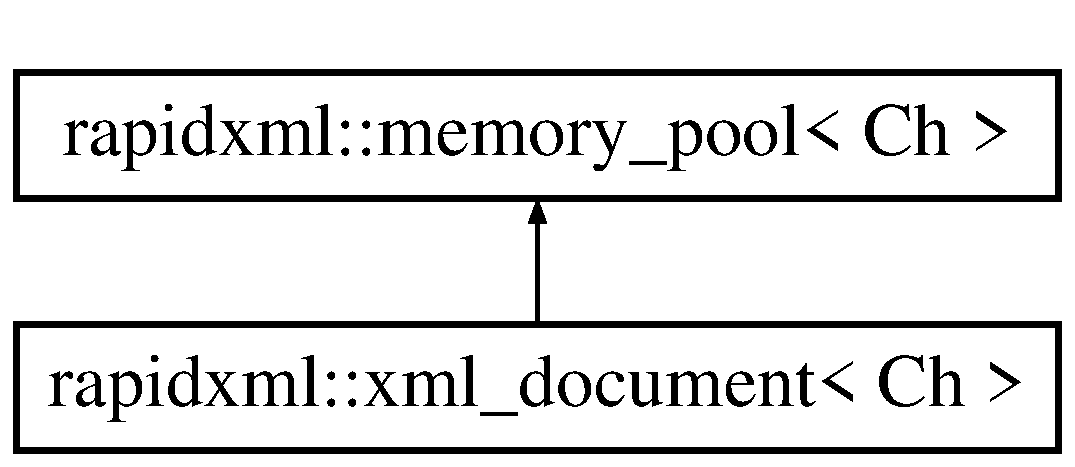
\includegraphics[height=2.000000cm]{classrapidxml_1_1memory__pool}
\end{center}
\end{figure}
\subsection*{Public Member Functions}
\begin{DoxyCompactItemize}
\item 
\hypertarget{classrapidxml_1_1memory__pool_a0b609da81dff28a19ebd704400788429}{\hyperlink{classrapidxml_1_1memory__pool_a0b609da81dff28a19ebd704400788429}{memory\+\_\+pool} ()}\label{classrapidxml_1_1memory__pool_a0b609da81dff28a19ebd704400788429}

\begin{DoxyCompactList}\small\item\em Constructs empty pool with default allocator functions. \end{DoxyCompactList}\item 
\hyperlink{classrapidxml_1_1memory__pool_a0a3e82126e59e4077f41e933130bb5a0}{$\sim$memory\+\_\+pool} ()
\item 
\hyperlink{singletonrapidxml_1_1xml__node}{xml\+\_\+node}$<$ Ch $>$ $\ast$ \hyperlink{classrapidxml_1_1memory__pool_a4118581c29ee9a2f6b55ebf7dac185f8}{allocate\+\_\+node} (node\+\_\+type type, const Ch $\ast$name=0, const Ch $\ast$value=0, std\+::size\+\_\+t name\+\_\+size=0, std\+::size\+\_\+t value\+\_\+size=0)
\item 
\hyperlink{singletonrapidxml_1_1xml__attribute}{xml\+\_\+attribute}$<$ Ch $>$ $\ast$ \hyperlink{classrapidxml_1_1memory__pool_a3de2a66c983336e006ea3844e244ed30}{allocate\+\_\+attribute} (const Ch $\ast$name=0, const Ch $\ast$value=0, std\+::size\+\_\+t name\+\_\+size=0, std\+::size\+\_\+t value\+\_\+size=0)
\item 
Ch $\ast$ \hyperlink{classrapidxml_1_1memory__pool_a171941b39d55b868358da97462185f58}{allocate\+\_\+string} (const Ch $\ast$source=0, std\+::size\+\_\+t size=0)
\item 
\hyperlink{singletonrapidxml_1_1xml__node}{xml\+\_\+node}$<$ Ch $>$ $\ast$ \hyperlink{classrapidxml_1_1memory__pool_a0a10679fc17597d339a0dc107f8a94ac}{clone\+\_\+node} (const \hyperlink{singletonrapidxml_1_1xml__node}{xml\+\_\+node}$<$ Ch $>$ $\ast$source, \hyperlink{singletonrapidxml_1_1xml__node}{xml\+\_\+node}$<$ Ch $>$ $\ast$result=0)
\item 
void \hyperlink{classrapidxml_1_1memory__pool_aad377c835fdaed1cb2cc9df194cf84e4}{clear} ()
\item 
void \hyperlink{classrapidxml_1_1memory__pool_a84d3d8d2cdfc00501e1dcf26d889ae03}{set\+\_\+allocator} (alloc\+\_\+func $\ast$af, free\+\_\+func $\ast$ff)
\end{DoxyCompactItemize}


\subsection{Detailed Description}
\subsubsection*{template$<$class Ch = char$>$class rapidxml\+::memory\+\_\+pool$<$ Ch $>$}

This class is used by the parser to create new nodes and attributes, without overheads of dynamic memory allocation. In most cases, you will not need to use this class directly. However, if you need to create nodes manually or modify names/values of nodes, you are encouraged to use \hyperlink{classrapidxml_1_1memory__pool}{memory\+\_\+pool} of relevant \hyperlink{singletonrapidxml_1_1xml__document}{xml\+\_\+document} to allocate the memory. Not only is this faster than allocating them by using {\ttfamily new} operator, but also their lifetime will be tied to the lifetime of document, possibly simplyfing memory management. ~\newline
~\newline
 Call \hyperlink{classrapidxml_1_1memory__pool_a4118581c29ee9a2f6b55ebf7dac185f8}{allocate\+\_\+node()} or \hyperlink{classrapidxml_1_1memory__pool_a3de2a66c983336e006ea3844e244ed30}{allocate\+\_\+attribute()} functions to obtain new nodes or attributes from the pool. You can also call \hyperlink{classrapidxml_1_1memory__pool_a171941b39d55b868358da97462185f58}{allocate\+\_\+string()} function to allocate strings. Such strings can then be used as names or values of nodes without worrying about their lifetime. Note that there is no {\ttfamily free()} function -- all allocations are freed at once when \hyperlink{classrapidxml_1_1memory__pool_aad377c835fdaed1cb2cc9df194cf84e4}{clear()} function is called, or when the pool is destroyed. ~\newline
~\newline
 It is also possible to create a standalone \hyperlink{classrapidxml_1_1memory__pool}{memory\+\_\+pool}, and use it to allocate nodes, whose lifetime will not be tied to any document. ~\newline
~\newline
 Pool maintains {\ttfamily R\+A\+P\+I\+D\+X\+M\+L\+\_\+\+S\+T\+A\+T\+I\+C\+\_\+\+P\+O\+O\+L\+\_\+\+S\+I\+Z\+E} bytes of statically allocated memory. Until static memory is exhausted, no dynamic memory allocations are done. When static memory is exhausted, pool allocates additional blocks of memory of size {\ttfamily R\+A\+P\+I\+D\+X\+M\+L\+\_\+\+D\+Y\+N\+A\+M\+I\+C\+\_\+\+P\+O\+O\+L\+\_\+\+S\+I\+Z\+E} each, by using global {\ttfamily new\mbox{[}\mbox{]}} and {\ttfamily delete\mbox{[}\mbox{]}} operators. This behaviour can be changed by setting custom allocation routines. Use \hyperlink{classrapidxml_1_1memory__pool_a84d3d8d2cdfc00501e1dcf26d889ae03}{set\+\_\+allocator()} function to set them. ~\newline
~\newline
 Allocations for nodes, attributes and strings are aligned at {\ttfamily R\+A\+P\+I\+D\+X\+M\+L\+\_\+\+A\+L\+I\+G\+N\+M\+E\+N\+T} bytes. This value defaults to the size of pointer on target architecture. ~\newline
~\newline
 To obtain absolutely top performance from the parser, it is important that all nodes are allocated from a single, contiguous block of memory. Otherwise, cache misses when jumping between two (or more) disjoint blocks of memory can slow down parsing quite considerably. If required, you can tweak {\ttfamily R\+A\+P\+I\+D\+X\+M\+L\+\_\+\+S\+T\+A\+T\+I\+C\+\_\+\+P\+O\+O\+L\+\_\+\+S\+I\+Z\+E}, {\ttfamily R\+A\+P\+I\+D\+X\+M\+L\+\_\+\+D\+Y\+N\+A\+M\+I\+C\+\_\+\+P\+O\+O\+L\+\_\+\+S\+I\+Z\+E} and {\ttfamily R\+A\+P\+I\+D\+X\+M\+L\+\_\+\+A\+L\+I\+G\+N\+M\+E\+N\+T} to obtain best wasted memory to performance compromise. To do it, define their values before \hyperlink{rapidxml_8hpp}{rapidxml.\+hpp} file is included. 
\begin{DoxyParams}{Parameters}
{\em Ch} & Character type of created nodes. \\
\hline
\end{DoxyParams}


\subsection{Constructor \& Destructor Documentation}
\hypertarget{classrapidxml_1_1memory__pool_a0a3e82126e59e4077f41e933130bb5a0}{\index{rapidxml\+::memory\+\_\+pool@{rapidxml\+::memory\+\_\+pool}!````~memory\+\_\+pool@{$\sim$memory\+\_\+pool}}
\index{````~memory\+\_\+pool@{$\sim$memory\+\_\+pool}!rapidxml\+::memory\+\_\+pool@{rapidxml\+::memory\+\_\+pool}}
\subsubsection[{$\sim$memory\+\_\+pool}]{\setlength{\rightskip}{0pt plus 5cm}template$<$class Ch  = char$>$ {\bf rapidxml\+::memory\+\_\+pool}$<$ Ch $>$\+::$\sim${\bf memory\+\_\+pool} (
\begin{DoxyParamCaption}
{}
\end{DoxyParamCaption}
)\hspace{0.3cm}{\ttfamily [inline]}}}\label{classrapidxml_1_1memory__pool_a0a3e82126e59e4077f41e933130bb5a0}
Destroys pool and frees all the memory. This causes memory occupied by nodes allocated by the pool to be freed. Nodes allocated from the pool are no longer valid. 

\subsection{Member Function Documentation}
\hypertarget{classrapidxml_1_1memory__pool_a3de2a66c983336e006ea3844e244ed30}{\index{rapidxml\+::memory\+\_\+pool@{rapidxml\+::memory\+\_\+pool}!allocate\+\_\+attribute@{allocate\+\_\+attribute}}
\index{allocate\+\_\+attribute@{allocate\+\_\+attribute}!rapidxml\+::memory\+\_\+pool@{rapidxml\+::memory\+\_\+pool}}
\subsubsection[{allocate\+\_\+attribute}]{\setlength{\rightskip}{0pt plus 5cm}template$<$class Ch  = char$>$ {\bf xml\+\_\+attribute}$<$Ch$>$$\ast$ {\bf rapidxml\+::memory\+\_\+pool}$<$ Ch $>$\+::allocate\+\_\+attribute (
\begin{DoxyParamCaption}
\item[{const Ch $\ast$}]{name = {\ttfamily 0}, }
\item[{const Ch $\ast$}]{value = {\ttfamily 0}, }
\item[{std\+::size\+\_\+t}]{name\+\_\+size = {\ttfamily 0}, }
\item[{std\+::size\+\_\+t}]{value\+\_\+size = {\ttfamily 0}}
\end{DoxyParamCaption}
)\hspace{0.3cm}{\ttfamily [inline]}}}\label{classrapidxml_1_1memory__pool_a3de2a66c983336e006ea3844e244ed30}
Allocates a new attribute from the pool, and optionally assigns name and value to it. If the allocation request cannot be accomodated, this function will throw {\ttfamily std\+::bad\+\_\+alloc}. If exceptions are disabled by defining R\+A\+P\+I\+D\+X\+M\+L\+\_\+\+N\+O\+\_\+\+E\+X\+C\+E\+P\+T\+I\+O\+N\+S, this function will call rapidxml\+::parse\+\_\+error\+\_\+handler() function. 
\begin{DoxyParams}{Parameters}
{\em name} & Name to assign to the attribute, or 0 to assign no name. \\
\hline
{\em value} & Value to assign to the attribute, or 0 to assign no value. \\
\hline
{\em name\+\_\+size} & Size of name to assign, or 0 to automatically calculate size from name string. \\
\hline
{\em value\+\_\+size} & Size of value to assign, or 0 to automatically calculate size from value string. \\
\hline
\end{DoxyParams}
\begin{DoxyReturn}{Returns}
Pointer to allocated attribute. This pointer will never be N\+U\+L\+L. 
\end{DoxyReturn}
\hypertarget{classrapidxml_1_1memory__pool_a4118581c29ee9a2f6b55ebf7dac185f8}{\index{rapidxml\+::memory\+\_\+pool@{rapidxml\+::memory\+\_\+pool}!allocate\+\_\+node@{allocate\+\_\+node}}
\index{allocate\+\_\+node@{allocate\+\_\+node}!rapidxml\+::memory\+\_\+pool@{rapidxml\+::memory\+\_\+pool}}
\subsubsection[{allocate\+\_\+node}]{\setlength{\rightskip}{0pt plus 5cm}template$<$class Ch  = char$>$ {\bf xml\+\_\+node}$<$Ch$>$$\ast$ {\bf rapidxml\+::memory\+\_\+pool}$<$ Ch $>$\+::allocate\+\_\+node (
\begin{DoxyParamCaption}
\item[{node\+\_\+type}]{type, }
\item[{const Ch $\ast$}]{name = {\ttfamily 0}, }
\item[{const Ch $\ast$}]{value = {\ttfamily 0}, }
\item[{std\+::size\+\_\+t}]{name\+\_\+size = {\ttfamily 0}, }
\item[{std\+::size\+\_\+t}]{value\+\_\+size = {\ttfamily 0}}
\end{DoxyParamCaption}
)\hspace{0.3cm}{\ttfamily [inline]}}}\label{classrapidxml_1_1memory__pool_a4118581c29ee9a2f6b55ebf7dac185f8}
Allocates a new node from the pool, and optionally assigns name and value to it. If the allocation request cannot be accomodated, this function will throw {\ttfamily std\+::bad\+\_\+alloc}. If exceptions are disabled by defining R\+A\+P\+I\+D\+X\+M\+L\+\_\+\+N\+O\+\_\+\+E\+X\+C\+E\+P\+T\+I\+O\+N\+S, this function will call rapidxml\+::parse\+\_\+error\+\_\+handler() function. 
\begin{DoxyParams}{Parameters}
{\em type} & Type of node to create. \\
\hline
{\em name} & Name to assign to the node, or 0 to assign no name. \\
\hline
{\em value} & Value to assign to the node, or 0 to assign no value. \\
\hline
{\em name\+\_\+size} & Size of name to assign, or 0 to automatically calculate size from name string. \\
\hline
{\em value\+\_\+size} & Size of value to assign, or 0 to automatically calculate size from value string. \\
\hline
\end{DoxyParams}
\begin{DoxyReturn}{Returns}
Pointer to allocated node. This pointer will never be N\+U\+L\+L. 
\end{DoxyReturn}
\hypertarget{classrapidxml_1_1memory__pool_a171941b39d55b868358da97462185f58}{\index{rapidxml\+::memory\+\_\+pool@{rapidxml\+::memory\+\_\+pool}!allocate\+\_\+string@{allocate\+\_\+string}}
\index{allocate\+\_\+string@{allocate\+\_\+string}!rapidxml\+::memory\+\_\+pool@{rapidxml\+::memory\+\_\+pool}}
\subsubsection[{allocate\+\_\+string}]{\setlength{\rightskip}{0pt plus 5cm}template$<$class Ch  = char$>$ Ch$\ast$ {\bf rapidxml\+::memory\+\_\+pool}$<$ Ch $>$\+::allocate\+\_\+string (
\begin{DoxyParamCaption}
\item[{const Ch $\ast$}]{source = {\ttfamily 0}, }
\item[{std\+::size\+\_\+t}]{size = {\ttfamily 0}}
\end{DoxyParamCaption}
)\hspace{0.3cm}{\ttfamily [inline]}}}\label{classrapidxml_1_1memory__pool_a171941b39d55b868358da97462185f58}
Allocates a char array of given size from the pool, and optionally copies a given string to it. If the allocation request cannot be accomodated, this function will throw {\ttfamily std\+::bad\+\_\+alloc}. If exceptions are disabled by defining R\+A\+P\+I\+D\+X\+M\+L\+\_\+\+N\+O\+\_\+\+E\+X\+C\+E\+P\+T\+I\+O\+N\+S, this function will call rapidxml\+::parse\+\_\+error\+\_\+handler() function. 
\begin{DoxyParams}{Parameters}
{\em source} & String to initialize the allocated memory with, or 0 to not initialize it. \\
\hline
{\em size} & Number of characters to allocate, or zero to calculate it automatically from source string length; if size is 0, source string must be specified and null terminated. \\
\hline
\end{DoxyParams}
\begin{DoxyReturn}{Returns}
Pointer to allocated char array. This pointer will never be N\+U\+L\+L. 
\end{DoxyReturn}
\hypertarget{classrapidxml_1_1memory__pool_aad377c835fdaed1cb2cc9df194cf84e4}{\index{rapidxml\+::memory\+\_\+pool@{rapidxml\+::memory\+\_\+pool}!clear@{clear}}
\index{clear@{clear}!rapidxml\+::memory\+\_\+pool@{rapidxml\+::memory\+\_\+pool}}
\subsubsection[{clear}]{\setlength{\rightskip}{0pt plus 5cm}template$<$class Ch  = char$>$ void {\bf rapidxml\+::memory\+\_\+pool}$<$ Ch $>$\+::clear (
\begin{DoxyParamCaption}
{}
\end{DoxyParamCaption}
)\hspace{0.3cm}{\ttfamily [inline]}}}\label{classrapidxml_1_1memory__pool_aad377c835fdaed1cb2cc9df194cf84e4}
Clears the pool. This causes memory occupied by nodes allocated by the pool to be freed. Any nodes or strings allocated from the pool will no longer be valid. \hypertarget{classrapidxml_1_1memory__pool_a0a10679fc17597d339a0dc107f8a94ac}{\index{rapidxml\+::memory\+\_\+pool@{rapidxml\+::memory\+\_\+pool}!clone\+\_\+node@{clone\+\_\+node}}
\index{clone\+\_\+node@{clone\+\_\+node}!rapidxml\+::memory\+\_\+pool@{rapidxml\+::memory\+\_\+pool}}
\subsubsection[{clone\+\_\+node}]{\setlength{\rightskip}{0pt plus 5cm}template$<$class Ch  = char$>$ {\bf xml\+\_\+node}$<$Ch$>$$\ast$ {\bf rapidxml\+::memory\+\_\+pool}$<$ Ch $>$\+::clone\+\_\+node (
\begin{DoxyParamCaption}
\item[{const {\bf xml\+\_\+node}$<$ Ch $>$ $\ast$}]{source, }
\item[{{\bf xml\+\_\+node}$<$ Ch $>$ $\ast$}]{result = {\ttfamily 0}}
\end{DoxyParamCaption}
)\hspace{0.3cm}{\ttfamily [inline]}}}\label{classrapidxml_1_1memory__pool_a0a10679fc17597d339a0dc107f8a94ac}
Clones an \hyperlink{singletonrapidxml_1_1xml__node}{xml\+\_\+node} and its hierarchy of child nodes and attributes. Nodes and attributes are allocated from this memory pool. Names and values are not cloned, they are shared between the clone and the source. Result node can be optionally specified as a second parameter, in which case its contents will be replaced with cloned source node. This is useful when you want to clone entire document. 
\begin{DoxyParams}{Parameters}
{\em source} & Node to clone. \\
\hline
{\em result} & Node to put results in, or 0 to automatically allocate result node \\
\hline
\end{DoxyParams}
\begin{DoxyReturn}{Returns}
Pointer to cloned node. This pointer will never be N\+U\+L\+L. 
\end{DoxyReturn}
\hypertarget{classrapidxml_1_1memory__pool_a84d3d8d2cdfc00501e1dcf26d889ae03}{\index{rapidxml\+::memory\+\_\+pool@{rapidxml\+::memory\+\_\+pool}!set\+\_\+allocator@{set\+\_\+allocator}}
\index{set\+\_\+allocator@{set\+\_\+allocator}!rapidxml\+::memory\+\_\+pool@{rapidxml\+::memory\+\_\+pool}}
\subsubsection[{set\+\_\+allocator}]{\setlength{\rightskip}{0pt plus 5cm}template$<$class Ch  = char$>$ void {\bf rapidxml\+::memory\+\_\+pool}$<$ Ch $>$\+::set\+\_\+allocator (
\begin{DoxyParamCaption}
\item[{alloc\+\_\+func $\ast$}]{af, }
\item[{free\+\_\+func $\ast$}]{ff}
\end{DoxyParamCaption}
)\hspace{0.3cm}{\ttfamily [inline]}}}\label{classrapidxml_1_1memory__pool_a84d3d8d2cdfc00501e1dcf26d889ae03}
Sets or resets the user-\/defined memory allocation functions for the pool. This can only be called when no memory is allocated from the pool yet, otherwise results are undefined. Allocation function must not return invalid pointer on failure. It should either throw, stop the program, or use {\ttfamily longjmp()} function to pass control to other place of program. If it returns invalid pointer, results are undefined. ~\newline
~\newline
 User defined allocation functions must have the following forms\+: ~\newline
{\ttfamily  ~\newline
void $\ast$allocate(std\+::size\+\_\+t size); ~\newline
void free(void $\ast$pointer); }~\newline
 
\begin{DoxyParams}{Parameters}
{\em af} & Allocation function, or 0 to restore default function \\
\hline
{\em ff} & Free function, or 0 to restore default function \\
\hline
\end{DoxyParams}


The documentation for this class was generated from the following file\+:\begin{DoxyCompactItemize}
\item 
\hyperlink{rapidxml_8hpp}{rapidxml.\+hpp}\end{DoxyCompactItemize}

\hypertarget{classrapidxml_1_1node__iterator}{\section{rapidxml\+:\+:node\+\_\+iterator$<$ Ch $>$ Class Template Reference}
\label{classrapidxml_1_1node__iterator}\index{rapidxml\+::node\+\_\+iterator$<$ Ch $>$@{rapidxml\+::node\+\_\+iterator$<$ Ch $>$}}
}


Iterator of child nodes of \hyperlink{singletonrapidxml_1_1xml__node}{xml\+\_\+node}.  




{\ttfamily \#include $<$rapidxml\+\_\+iterators.\+hpp$>$}

\subsection*{Public Types}
\begin{DoxyCompactItemize}
\item 
\hypertarget{classrapidxml_1_1node__iterator_ade6310119ed1f72c94830e006fac69b7}{typedef \hyperlink{singletonrapidxml_1_1xml__node}{xml\+\_\+node}$<$ Ch $>$ {\bfseries value\+\_\+type}}\label{classrapidxml_1_1node__iterator_ade6310119ed1f72c94830e006fac69b7}

\item 
\hypertarget{classrapidxml_1_1node__iterator_ad7fabbcb7d3d9e4e220299c5475b9e9c}{typedef \hyperlink{singletonrapidxml_1_1xml__node}{xml\+\_\+node}$<$ Ch $>$ \& {\bfseries reference}}\label{classrapidxml_1_1node__iterator_ad7fabbcb7d3d9e4e220299c5475b9e9c}

\item 
\hypertarget{classrapidxml_1_1node__iterator_a65dca8bca2b9c29f635b9ad0bdeeecb9}{typedef \hyperlink{singletonrapidxml_1_1xml__node}{xml\+\_\+node}$<$ Ch $>$ $\ast$ {\bfseries pointer}}\label{classrapidxml_1_1node__iterator_a65dca8bca2b9c29f635b9ad0bdeeecb9}

\item 
\hypertarget{classrapidxml_1_1node__iterator_a5bdc462b980a52c5fa2d99ac9f4f4bff}{typedef std\+::ptrdiff\+\_\+t {\bfseries difference\+\_\+type}}\label{classrapidxml_1_1node__iterator_a5bdc462b980a52c5fa2d99ac9f4f4bff}

\item 
\hypertarget{classrapidxml_1_1node__iterator_a8e82d75f768e17bf7349d010ee26c037}{typedef \\*
std\+::bidirectional\+\_\+iterator\+\_\+tag {\bfseries iterator\+\_\+category}}\label{classrapidxml_1_1node__iterator_a8e82d75f768e17bf7349d010ee26c037}

\end{DoxyCompactItemize}
\subsection*{Public Member Functions}
\begin{DoxyCompactItemize}
\item 
\hypertarget{classrapidxml_1_1node__iterator_a94c3da59b54e4bd003e226cc35b3c266}{{\bfseries node\+\_\+iterator} (\hyperlink{singletonrapidxml_1_1xml__node}{xml\+\_\+node}$<$ Ch $>$ $\ast$node)}\label{classrapidxml_1_1node__iterator_a94c3da59b54e4bd003e226cc35b3c266}

\item 
\hypertarget{classrapidxml_1_1node__iterator_ab31fe5bc1fd01fee8a2b31c3e42d78ed}{\hyperlink{singletonrapidxml_1_1xml__node}{reference} {\bfseries operator$\ast$} () const }\label{classrapidxml_1_1node__iterator_ab31fe5bc1fd01fee8a2b31c3e42d78ed}

\item 
\hypertarget{classrapidxml_1_1node__iterator_a9b3e7d58c4a628524914932e0663ddfb}{\hyperlink{singletonrapidxml_1_1xml__node}{pointer} {\bfseries operator-\/$>$} () const }\label{classrapidxml_1_1node__iterator_a9b3e7d58c4a628524914932e0663ddfb}

\item 
\hypertarget{classrapidxml_1_1node__iterator_a8d6b184a76b2ec8a8b5e90bc013c80ed}{\hyperlink{classrapidxml_1_1node__iterator}{node\+\_\+iterator} \& {\bfseries operator++} ()}\label{classrapidxml_1_1node__iterator_a8d6b184a76b2ec8a8b5e90bc013c80ed}

\item 
\hypertarget{classrapidxml_1_1node__iterator_ad01b4e43e348a330984833fd4924d0f2}{\hyperlink{classrapidxml_1_1node__iterator}{node\+\_\+iterator} {\bfseries operator++} (int)}\label{classrapidxml_1_1node__iterator_ad01b4e43e348a330984833fd4924d0f2}

\item 
\hypertarget{classrapidxml_1_1node__iterator_ace52107ecd1bcf02e49619e86206e3a3}{\hyperlink{classrapidxml_1_1node__iterator}{node\+\_\+iterator} \& {\bfseries operator-\/-\/} ()}\label{classrapidxml_1_1node__iterator_ace52107ecd1bcf02e49619e86206e3a3}

\item 
\hypertarget{classrapidxml_1_1node__iterator_a4ca35716bb7865f199a137b063af6080}{\hyperlink{classrapidxml_1_1node__iterator}{node\+\_\+iterator} {\bfseries operator-\/-\/} (int)}\label{classrapidxml_1_1node__iterator_a4ca35716bb7865f199a137b063af6080}

\item 
\hypertarget{classrapidxml_1_1node__iterator_a5cb8a3b0d65a1a2517995e986a4debfd}{bool {\bfseries operator==} (const \hyperlink{classrapidxml_1_1node__iterator}{node\+\_\+iterator}$<$ Ch $>$ \&rhs)}\label{classrapidxml_1_1node__iterator_a5cb8a3b0d65a1a2517995e986a4debfd}

\item 
\hypertarget{classrapidxml_1_1node__iterator_a20f1e25347d7e3856694f18597f7c8e2}{bool {\bfseries operator!=} (const \hyperlink{classrapidxml_1_1node__iterator}{node\+\_\+iterator}$<$ Ch $>$ \&rhs)}\label{classrapidxml_1_1node__iterator_a20f1e25347d7e3856694f18597f7c8e2}

\end{DoxyCompactItemize}


\subsection{Detailed Description}
\subsubsection*{template$<$class Ch$>$class rapidxml\+::node\+\_\+iterator$<$ Ch $>$}

Iterator of child nodes of \hyperlink{singletonrapidxml_1_1xml__node}{xml\+\_\+node}. 

The documentation for this class was generated from the following file\+:\begin{DoxyCompactItemize}
\item 
\hyperlink{rapidxml__iterators_8hpp}{rapidxml\+\_\+iterators.\+hpp}\end{DoxyCompactItemize}

\hypertarget{classrapidxml_1_1parse__error}{\section{rapidxml\+:\+:parse\+\_\+error Class Reference}
\label{classrapidxml_1_1parse__error}\index{rapidxml\+::parse\+\_\+error@{rapidxml\+::parse\+\_\+error}}
}


{\ttfamily \#include $<$rapidxml.\+hpp$>$}

Inheritance diagram for rapidxml\+:\+:parse\+\_\+error\+:\begin{figure}[H]
\begin{center}
\leavevmode
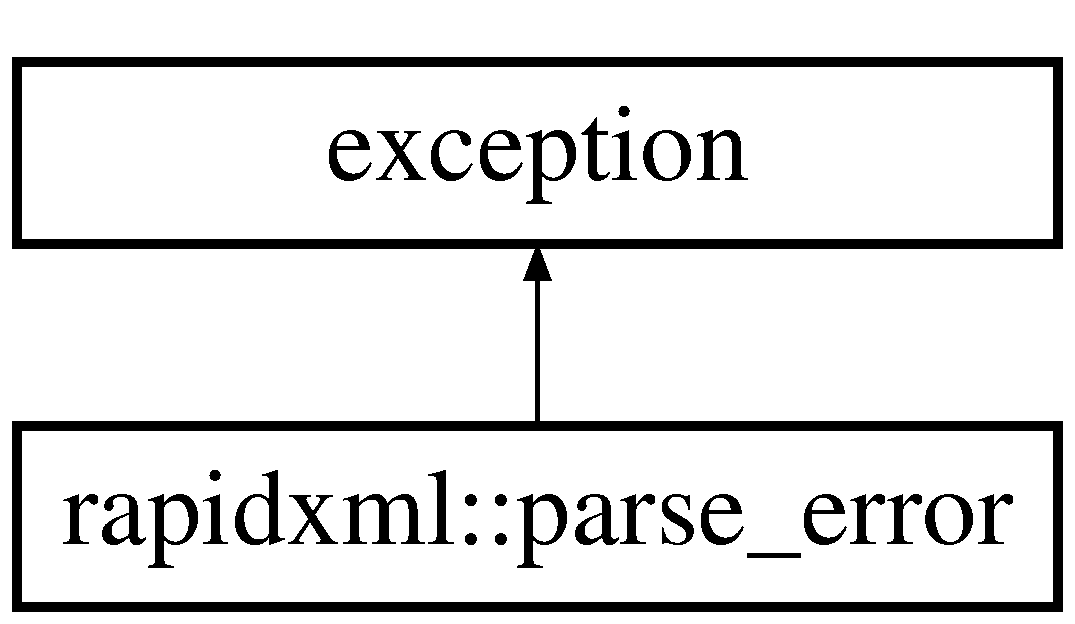
\includegraphics[height=2.000000cm]{classrapidxml_1_1parse__error}
\end{center}
\end{figure}
\subsection*{Public Member Functions}
\begin{DoxyCompactItemize}
\item 
\hypertarget{classrapidxml_1_1parse__error_aea12a301271c393fb627b368fb9f35c1}{\hyperlink{classrapidxml_1_1parse__error_aea12a301271c393fb627b368fb9f35c1}{parse\+\_\+error} (const char $\ast$\hyperlink{classrapidxml_1_1parse__error_a7665c88639e7466ee1de388a4f85e6fe}{what}, void $\ast$\hyperlink{classrapidxml_1_1parse__error_a3a0ab9e586c1d2b437c340f6622fbec6}{where})}\label{classrapidxml_1_1parse__error_aea12a301271c393fb627b368fb9f35c1}

\begin{DoxyCompactList}\small\item\em Constructs parse error. \end{DoxyCompactList}\item 
virtual const char $\ast$ \hyperlink{classrapidxml_1_1parse__error_a7665c88639e7466ee1de388a4f85e6fe}{what} () const   throw ()
\item 
{\footnotesize template$<$class Ch $>$ }\\Ch $\ast$ \hyperlink{classrapidxml_1_1parse__error_a3a0ab9e586c1d2b437c340f6622fbec6}{where} () const 
\end{DoxyCompactItemize}


\subsection{Detailed Description}
Parse error exception. This exception is thrown by the parser when an error occurs. Use \hyperlink{classrapidxml_1_1parse__error_a7665c88639e7466ee1de388a4f85e6fe}{what()} function to get human-\/readable error message. Use \hyperlink{classrapidxml_1_1parse__error_a3a0ab9e586c1d2b437c340f6622fbec6}{where()} function to get a pointer to position within source text where error was detected. ~\newline
~\newline
 If throwing exceptions by the parser is undesirable, it can be disabled by defining R\+A\+P\+I\+D\+X\+M\+L\+\_\+\+N\+O\+\_\+\+E\+X\+C\+E\+P\+T\+I\+O\+N\+S macro before \hyperlink{rapidxml_8hpp}{rapidxml.\+hpp} is included. This will cause the parser to call rapidxml\+::parse\+\_\+error\+\_\+handler() function instead of throwing an exception. This function must be defined by the user. ~\newline
~\newline
 This class derives from {\ttfamily std\+::exception} class. 

\subsection{Member Function Documentation}
\hypertarget{classrapidxml_1_1parse__error_a7665c88639e7466ee1de388a4f85e6fe}{\index{rapidxml\+::parse\+\_\+error@{rapidxml\+::parse\+\_\+error}!what@{what}}
\index{what@{what}!rapidxml\+::parse\+\_\+error@{rapidxml\+::parse\+\_\+error}}
\subsubsection[{what}]{\setlength{\rightskip}{0pt plus 5cm}virtual const char$\ast$ rapidxml\+::parse\+\_\+error\+::what (
\begin{DoxyParamCaption}
{}
\end{DoxyParamCaption}
) const throw  ) \hspace{0.3cm}{\ttfamily [inline]}, {\ttfamily [virtual]}}}\label{classrapidxml_1_1parse__error_a7665c88639e7466ee1de388a4f85e6fe}
Gets human readable description of error. \begin{DoxyReturn}{Returns}
Pointer to null terminated description of the error. 
\end{DoxyReturn}
\hypertarget{classrapidxml_1_1parse__error_a3a0ab9e586c1d2b437c340f6622fbec6}{\index{rapidxml\+::parse\+\_\+error@{rapidxml\+::parse\+\_\+error}!where@{where}}
\index{where@{where}!rapidxml\+::parse\+\_\+error@{rapidxml\+::parse\+\_\+error}}
\subsubsection[{where}]{\setlength{\rightskip}{0pt plus 5cm}template$<$class Ch $>$ Ch$\ast$ rapidxml\+::parse\+\_\+error\+::where (
\begin{DoxyParamCaption}
{}
\end{DoxyParamCaption}
) const\hspace{0.3cm}{\ttfamily [inline]}}}\label{classrapidxml_1_1parse__error_a3a0ab9e586c1d2b437c340f6622fbec6}
Gets pointer to character data where error happened. Ch should be the same as char type of \hyperlink{singletonrapidxml_1_1xml__document}{xml\+\_\+document} that produced the error. \begin{DoxyReturn}{Returns}
Pointer to location within the parsed string where error occured. 
\end{DoxyReturn}


The documentation for this class was generated from the following file\+:\begin{DoxyCompactItemize}
\item 
\hyperlink{rapidxml_8hpp}{rapidxml.\+hpp}\end{DoxyCompactItemize}

\hypertarget{class_query_processor}{\section{Query\+Processor Class Reference}
\label{class_query_processor}\index{Query\+Processor@{Query\+Processor}}
}
\subsection*{Public Member Functions}
\begin{DoxyCompactItemize}
\item 
\hypertarget{class_query_processor_a03dd195b55e8e1ac8feebc6021459f88}{void {\bfseries establish\+Index} ()}\label{class_query_processor_a03dd195b55e8e1ac8feebc6021459f88}

\item 
\hypertarget{class_query_processor_a42b22f3d69b6fefa6dd69c2caa03144a}{void {\bfseries add\+New\+File} (const char $\ast$file\+Name)}\label{class_query_processor_a42b22f3d69b6fefa6dd69c2caa03144a}

\item 
\hypertarget{class_query_processor_a0aeeb78c270fd6b8f5c807c7c0022aed}{void {\bfseries process\+Manager} (int Query\+Type)}\label{class_query_processor_a0aeeb78c270fd6b8f5c807c7c0022aed}

\item 
\hypertarget{class_query_processor_a2f136e04a7198ef8455d8c3414d998e1}{\hyperlink{classunique_words}{unique\+Words} {\bfseries return\+And\+Query} (stringstream \&word\+List)}\label{class_query_processor_a2f136e04a7198ef8455d8c3414d998e1}

\item 
\hypertarget{class_query_processor_a4d265cc7dc3575330a965bd4ad41f016}{string {\bfseries return\+Single\+Query} (stringstream \&word\+List)}\label{class_query_processor_a4d265cc7dc3575330a965bd4ad41f016}

\item 
\hypertarget{class_query_processor_ac35ae179a5233776914c25a28738777f}{\hyperlink{classunique_words}{unique\+Words} {\bfseries return\+Or\+Query} (stringstream \&word\+List)}\label{class_query_processor_ac35ae179a5233776914c25a28738777f}

\item 
\hypertarget{class_query_processor_ac1231d6dc8be7ecf1855c1501f006e64}{void {\bfseries remove\+Not\+Query} (string \&not\+Word, stringstream \&to\+Be\+Cleaned)}\label{class_query_processor_ac1231d6dc8be7ecf1855c1501f006e64}

\end{DoxyCompactItemize}


The documentation for this class was generated from the following files\+:\begin{DoxyCompactItemize}
\item 
Query\+Processor.\+h\item 
Query\+Processor.\+cpp\end{DoxyCompactItemize}

\hypertarget{classstop_worder}{\section{stop\+Worder Class Reference}
\label{classstop_worder}\index{stop\+Worder@{stop\+Worder}}
}
\subsection*{Public Member Functions}
\begin{DoxyCompactItemize}
\item 
\hypertarget{classstop_worder_ad3a78eea2bf46b9f470267a4e7080f8d}{void {\bfseries load\+Stop\+Words} ()}\label{classstop_worder_ad3a78eea2bf46b9f470267a4e7080f8d}

\item 
\hypertarget{classstop_worder_a8fc9aae41e9744a89e491aa794e3c4b7}{std\+::string {\bfseries remove\+Stop\+Words} (std\+::stringstream \&word\+List)}\label{classstop_worder_a8fc9aae41e9744a89e491aa794e3c4b7}

\item 
\hypertarget{classstop_worder_a0d8447c55b750bb1929524d0d9817f31}{bool {\bfseries check\+If\+Stop} (std\+::string word)}\label{classstop_worder_a0d8447c55b750bb1929524d0d9817f31}

\item 
\hypertarget{classstop_worder_ad9155d34060767386dcb06dec394b56a}{bool {\bfseries punctuation\+Check} (char letter)}\label{classstop_worder_ad9155d34060767386dcb06dec394b56a}

\item 
\hypertarget{classstop_worder_a4275303ee66baeec417464b35e335345}{void {\bfseries check\+If\+Loaded} ()}\label{classstop_worder_a4275303ee66baeec417464b35e335345}

\item 
\hypertarget{classstop_worder_afa06f9295c87260f5175962a7c321806}{void {\bfseries clean} (string \&s)}\label{classstop_worder_afa06f9295c87260f5175962a7c321806}

\end{DoxyCompactItemize}


The documentation for this class was generated from the following files\+:\begin{DoxyCompactItemize}
\item 
Stop\+Worder.\+h\item 
Stop\+Worder.\+cpp\end{DoxyCompactItemize}

\hypertarget{classunique_words}{\section{unique\+Words Class Reference}
\label{classunique_words}\index{unique\+Words@{unique\+Words}}
}
\subsection*{Public Member Functions}
\begin{DoxyCompactItemize}
\item 
\hypertarget{classunique_words_a1124f70d6b94a791a5c53f1188c75c2c}{{\bfseries unique\+Words} (const \hyperlink{classunique_words}{unique\+Words} \&word)}\label{classunique_words_a1124f70d6b94a791a5c53f1188c75c2c}

\item 
\hypertarget{classunique_words_a964ba0558cded02ecf8c1f33ebb4bc9c}{{\bfseries unique\+Words} (string s)}\label{classunique_words_a964ba0558cded02ecf8c1f33ebb4bc9c}

\item 
\hypertarget{classunique_words_ae67a24b7a951cb687eda75cb4f630fca}{void {\bfseries set\+Name} (string s)}\label{classunique_words_ae67a24b7a951cb687eda75cb4f630fca}

\item 
\hypertarget{classunique_words_a7098dbeeca0a8963f873020b79789f71}{string {\bfseries get\+Name} ()}\label{classunique_words_a7098dbeeca0a8963f873020b79789f71}

\item 
\hypertarget{classunique_words_ad23a8595adf31b4ffcc8149efa510630}{void {\bfseries increment\+I\+D} (string S\+H\+A1)}\label{classunique_words_ad23a8595adf31b4ffcc8149efa510630}

\item 
\hypertarget{classunique_words_a3fc6e0c178048c2870ec34e07a783827}{void {\bfseries set\+Doc\+Freq\+Pair} (string str, int freq, int page\+Num=0)}\label{classunique_words_a3fc6e0c178048c2870ec34e07a783827}

\item 
\hypertarget{classunique_words_aade17e58ba6e3be3e8da501e9822e095}{\hyperlink{classunique_words}{unique\+Words} \& {\bfseries operator+=} (const \hyperlink{classunique_words}{unique\+Words} \&rhs)}\label{classunique_words_aade17e58ba6e3be3e8da501e9822e095}

\item 
\hypertarget{classunique_words_a7829d2c85feec32c833251b4b9931913}{\hyperlink{class_a_v_l_tree}{A\+V\+L\+Tree}$<$ \hyperlink{class_word_info}{Word\+Info} $>$ {\bfseries get\+Doc\+Freq\+Pairs} ()}\label{classunique_words_a7829d2c85feec32c833251b4b9931913}

\end{DoxyCompactItemize}
\subsection*{Friends}
\begin{DoxyCompactItemize}
\item 
\hypertarget{classunique_words_af3ed50cf61bd932ffc5e2bfe7e29c0ba}{bool {\bfseries operator==} (const \hyperlink{classunique_words}{unique\+Words} \&first, const \hyperlink{classunique_words}{unique\+Words} \&second)}\label{classunique_words_af3ed50cf61bd932ffc5e2bfe7e29c0ba}

\item 
\hypertarget{classunique_words_a0ea90430d23ca61da90502d8005ee1f4}{bool {\bfseries operator$<$} (const \hyperlink{classunique_words}{unique\+Words} \&first, const \hyperlink{classunique_words}{unique\+Words} \&second)}\label{classunique_words_a0ea90430d23ca61da90502d8005ee1f4}

\item 
\hypertarget{classunique_words_a6e99568e63a3985ccaa4222798d643c7}{bool {\bfseries operator$>$} (const \hyperlink{classunique_words}{unique\+Words} \&first, const \hyperlink{classunique_words}{unique\+Words} \&second)}\label{classunique_words_a6e99568e63a3985ccaa4222798d643c7}

\item 
\hypertarget{classunique_words_ad6afc81cc3346922a1f84d5e2b134325}{std\+::ostream \& {\bfseries operator$<$$<$} (std\+::ostream \&os, const \hyperlink{classunique_words}{unique\+Words} \&obj)}\label{classunique_words_ad6afc81cc3346922a1f84d5e2b134325}

\end{DoxyCompactItemize}


The documentation for this class was generated from the following files\+:\begin{DoxyCompactItemize}
\item 
unique\+Words.\+h\item 
unique\+Words.\+cpp\end{DoxyCompactItemize}

\hypertarget{class_virtual_indexer}{\section{Virtual\+Indexer Class Reference}
\label{class_virtual_indexer}\index{Virtual\+Indexer@{Virtual\+Indexer}}
}
Inheritance diagram for Virtual\+Indexer\+:\begin{figure}[H]
\begin{center}
\leavevmode
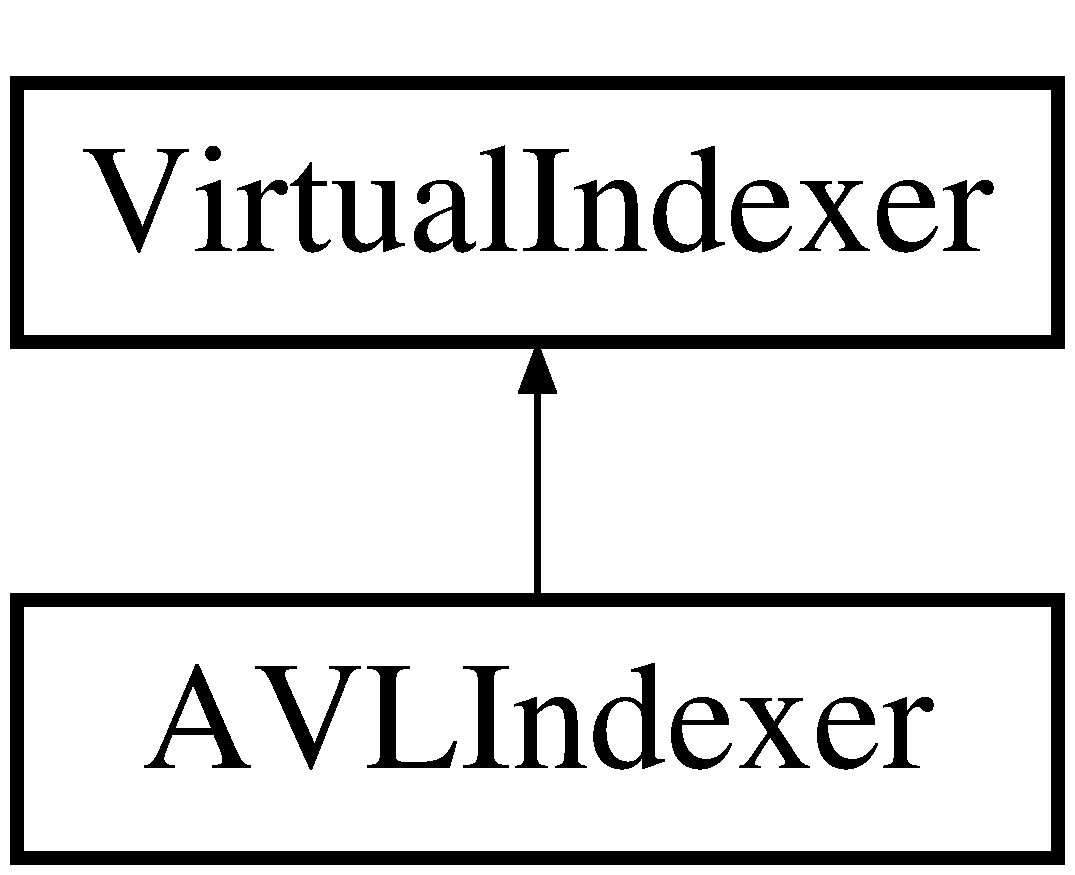
\includegraphics[height=2.000000cm]{class_virtual_indexer}
\end{center}
\end{figure}
\subsection*{Public Member Functions}
\begin{DoxyCompactItemize}
\item 
\hypertarget{class_virtual_indexer_a0630edbf3b068b8ad965025f61bc665b}{virtual void {\bfseries insert} (string word, string S\+H\+A1id, int frequency, int page\+Num)=0}\label{class_virtual_indexer_a0630edbf3b068b8ad965025f61bc665b}

\item 
\hypertarget{class_virtual_indexer_a24d704d5f93194c9049312f22af38637}{virtual \hyperlink{class_a_v_l_tree}{A\+V\+L\+Tree}$<$ \hyperlink{class_word_info}{Word\+Info} $>$ {\bfseries search} (string word)=0}\label{class_virtual_indexer_a24d704d5f93194c9049312f22af38637}

\item 
\hypertarget{class_virtual_indexer_a0f0b049e96a7fa3db62eac06d3d6c9d4}{virtual void {\bfseries delete\+Index} ()=0}\label{class_virtual_indexer_a0f0b049e96a7fa3db62eac06d3d6c9d4}

\item 
\hypertarget{class_virtual_indexer_a1cfb2760b2f51d21671b1c3fa1680171}{virtual void {\bfseries save\+Index} ()=0}\label{class_virtual_indexer_a1cfb2760b2f51d21671b1c3fa1680171}

\item 
\hypertarget{class_virtual_indexer_a4fcc7182a66a4e5c5d487043b3b638c2}{virtual void {\bfseries print\+Index} (ostream \&ostrm)=0}\label{class_virtual_indexer_a4fcc7182a66a4e5c5d487043b3b638c2}

\item 
\hypertarget{class_virtual_indexer_aafb98704c4cccc89b718a824c60c8360}{virtual bool {\bfseries is\+Found} (string word)=0}\label{class_virtual_indexer_aafb98704c4cccc89b718a824c60c8360}

\item 
\hypertarget{class_virtual_indexer_aa3b42a4556152954840137864b892315}{virtual void {\bfseries increment\+Frequency} (string word, string S\+H\+A1, int freq)=0}\label{class_virtual_indexer_aa3b42a4556152954840137864b892315}

\end{DoxyCompactItemize}


The documentation for this class was generated from the following files\+:\begin{DoxyCompactItemize}
\item 
Virtual\+Indexer.\+h\item 
Virtual\+Indexer.\+cpp\end{DoxyCompactItemize}

\hypertarget{class_word_info}{\section{Word\+Info Class Reference}
\label{class_word_info}\index{Word\+Info@{Word\+Info}}
}
\subsection*{Public Member Functions}
\begin{DoxyCompactItemize}
\item 
\hypertarget{class_word_info_af7a9b9d57364ecdfbfb57e75bdba892b}{{\bfseries Word\+Info} (const \hyperlink{class_word_info}{Word\+Info} \&word\+Info)}\label{class_word_info_af7a9b9d57364ecdfbfb57e75bdba892b}

\item 
\hypertarget{class_word_info_a35939caf471e57448e70c4f5b03f6029}{{\bfseries Word\+Info} (string s)}\label{class_word_info_a35939caf471e57448e70c4f5b03f6029}

\item 
\hypertarget{class_word_info_abd1c765dd61733c197611f4dcc85836c}{{\bfseries Word\+Info} (int f, int n, string s)}\label{class_word_info_abd1c765dd61733c197611f4dcc85836c}

\item 
\hypertarget{class_word_info_af2ee9869a097d5ef78a551f79f99ee39}{void {\bfseries set\+Freq} (int i)}\label{class_word_info_af2ee9869a097d5ef78a551f79f99ee39}

\item 
\hypertarget{class_word_info_adaacce5cd71311322732f1089026b281}{void {\bfseries set\+Page\+Num} (int i)}\label{class_word_info_adaacce5cd71311322732f1089026b281}

\item 
\hypertarget{class_word_info_a68f673ad022ff19bc86b1521bdbb536f}{void {\bfseries set\+S\+H\+A1} (string s)}\label{class_word_info_a68f673ad022ff19bc86b1521bdbb536f}

\item 
\hypertarget{class_word_info_a160c795ff8b17299525581c4b4bb65d6}{void {\bfseries increment} ()}\label{class_word_info_a160c795ff8b17299525581c4b4bb65d6}

\item 
\hypertarget{class_word_info_a2a40070a68e6cfbb3e3087c6642ac86c}{string {\bfseries get\+Obj\+Info} () const }\label{class_word_info_a2a40070a68e6cfbb3e3087c6642ac86c}

\item 
\hypertarget{class_word_info_ac4313e54d4d90e6e3a90a22e7e27c289}{\hyperlink{class_word_info}{Word\+Info} \& {\bfseries operator+=} (const \hyperlink{class_word_info}{Word\+Info} \&rhs)}\label{class_word_info_ac4313e54d4d90e6e3a90a22e7e27c289}

\end{DoxyCompactItemize}
\subsection*{Friends}
\begin{DoxyCompactItemize}
\item 
\hypertarget{class_word_info_a4c30cf1518b558337253b945ccd521d2}{bool {\bfseries operator$<$} (const \hyperlink{class_word_info}{Word\+Info} \&lhs, const \hyperlink{class_word_info}{Word\+Info} \&rhs)}\label{class_word_info_a4c30cf1518b558337253b945ccd521d2}

\item 
\hypertarget{class_word_info_a4bf92b0be09436e748a36f358f84d734}{bool {\bfseries operator==} (const \hyperlink{class_word_info}{Word\+Info} \&lhs, const \hyperlink{class_word_info}{Word\+Info} \&rhs)}\label{class_word_info_a4bf92b0be09436e748a36f358f84d734}

\item 
\hypertarget{class_word_info_ad5be93424e25e9468002e7514be32363}{bool {\bfseries operator==} (const \hyperlink{class_word_info}{Word\+Info} \&lhs, const string \&rhs)}\label{class_word_info_ad5be93424e25e9468002e7514be32363}

\item 
\hypertarget{class_word_info_aba1f3f7387dd5574e1e9c787943c75e9}{bool {\bfseries operator$>$} (const \hyperlink{class_word_info}{Word\+Info} \&lhs, const \hyperlink{class_word_info}{Word\+Info} \&rhs)}\label{class_word_info_aba1f3f7387dd5574e1e9c787943c75e9}

\item 
\hypertarget{class_word_info_accc174cc916eae2e7e7016522097976d}{std\+::ostream \& {\bfseries operator$<$$<$} (std\+::ostream \&os, const \hyperlink{class_word_info}{Word\+Info} \&obj)}\label{class_word_info_accc174cc916eae2e7e7016522097976d}

\end{DoxyCompactItemize}


The documentation for this class was generated from the following files\+:\begin{DoxyCompactItemize}
\item 
Word\+Info.\+h\item 
Word\+Info.\+cpp\end{DoxyCompactItemize}

\hypertarget{singletonrapidxml_1_1xml__attribute}{\section{rapidxml\+:\+:xml\+\_\+attribute$<$ Ch $>$ Class Template Reference}
\label{singletonrapidxml_1_1xml__attribute}\index{rapidxml\+::xml\+\_\+attribute$<$ Ch $>$@{rapidxml\+::xml\+\_\+attribute$<$ Ch $>$}}
}


{\ttfamily \#include $<$rapidxml.\+hpp$>$}

Inheritance diagram for rapidxml\+:\+:xml\+\_\+attribute$<$ Ch $>$\+:\begin{figure}[H]
\begin{center}
\leavevmode
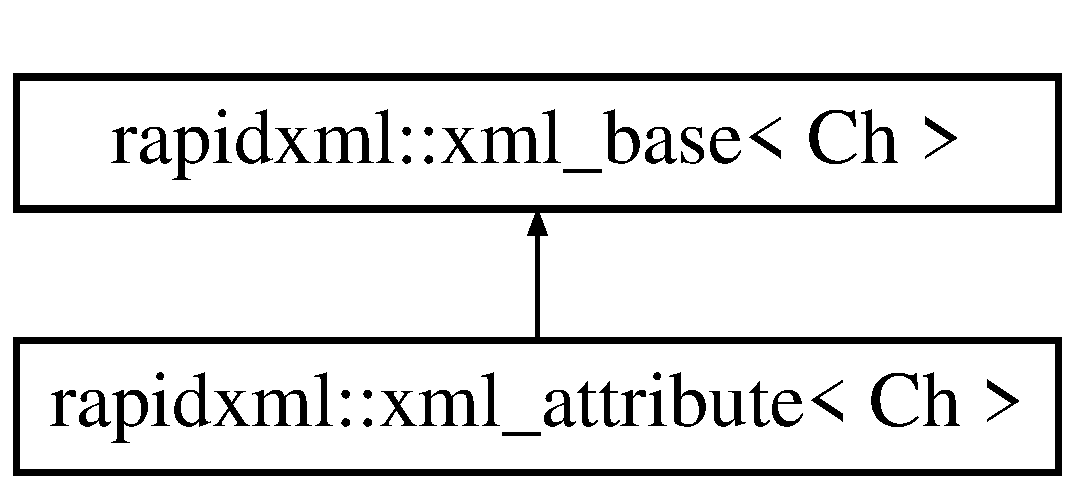
\includegraphics[height=2.000000cm]{singletonrapidxml_1_1xml__attribute}
\end{center}
\end{figure}
\subsection*{Public Member Functions}
\begin{DoxyCompactItemize}
\item 
\hyperlink{singletonrapidxml_1_1xml__attribute_a26be291103917d3e8de110d46dd83816}{xml\+\_\+attribute} ()
\item 
\hyperlink{singletonrapidxml_1_1xml__document}{xml\+\_\+document}$<$ Ch $>$ $\ast$ \hyperlink{singletonrapidxml_1_1xml__attribute_a8b6d31d899e27f01bde35b53d98496ec}{document} () const 
\item 
\hyperlink{singletonrapidxml_1_1xml__attribute}{xml\+\_\+attribute}$<$ Ch $>$ $\ast$ \hyperlink{singletonrapidxml_1_1xml__attribute_ae3547cc30b201fd6d7b98c04dda26f89}{previous\+\_\+attribute} (const Ch $\ast$\hyperlink{classrapidxml_1_1xml__base_a9a09739310469995db078ebd0da3ed45}{name}=0, std\+::size\+\_\+t \hyperlink{classrapidxml_1_1xml__base_a7e7f98b3d01e1eab8dc1ca69aad9af84}{name\+\_\+size}=0, bool case\+\_\+sensitive=true) const 
\item 
\hyperlink{singletonrapidxml_1_1xml__attribute}{xml\+\_\+attribute}$<$ Ch $>$ $\ast$ \hyperlink{singletonrapidxml_1_1xml__attribute_a56c08d7c96203286c889a43849328a86}{next\+\_\+attribute} (const Ch $\ast$\hyperlink{classrapidxml_1_1xml__base_a9a09739310469995db078ebd0da3ed45}{name}=0, std\+::size\+\_\+t \hyperlink{classrapidxml_1_1xml__base_a7e7f98b3d01e1eab8dc1ca69aad9af84}{name\+\_\+size}=0, bool case\+\_\+sensitive=true) const 
\end{DoxyCompactItemize}
\subsection*{Friends}
\begin{DoxyCompactItemize}
\item 
\hypertarget{singletonrapidxml_1_1xml__attribute_aa7e464ce3fe512598ff8dda47291941f}{class {\bfseries xml\+\_\+node$<$ Ch $>$}}\label{singletonrapidxml_1_1xml__attribute_aa7e464ce3fe512598ff8dda47291941f}

\end{DoxyCompactItemize}
\subsection*{Additional Inherited Members}


\subsection{Detailed Description}
\subsubsection*{template$<$class Ch = char$>$class rapidxml\+::xml\+\_\+attribute$<$ Ch $>$}

Class representing attribute node of X\+M\+L document. Each attribute has name and value strings, which are available through \hyperlink{classrapidxml_1_1xml__base_a9a09739310469995db078ebd0da3ed45}{name()} and \hyperlink{classrapidxml_1_1xml__base_adcdaccff61c665f039d9344e447b7445}{value()} functions (inherited from \hyperlink{classrapidxml_1_1xml__base}{xml\+\_\+base}). Note that after parse, both name and value of attribute will point to interior of source text used for parsing. Thus, this text must persist in memory for the lifetime of attribute. 
\begin{DoxyParams}{Parameters}
{\em Ch} & Character type to use. \\
\hline
\end{DoxyParams}


\subsection{Constructor \& Destructor Documentation}
\hypertarget{singletonrapidxml_1_1xml__attribute_a26be291103917d3e8de110d46dd83816}{\index{rapidxml\+::xml\+\_\+attribute@{rapidxml\+::xml\+\_\+attribute}!xml\+\_\+attribute@{xml\+\_\+attribute}}
\index{xml\+\_\+attribute@{xml\+\_\+attribute}!rapidxml\+::xml\+\_\+attribute@{rapidxml\+::xml\+\_\+attribute}}
\subsubsection[{xml\+\_\+attribute}]{\setlength{\rightskip}{0pt plus 5cm}template$<$class Ch = char$>$ {\bf rapidxml\+::xml\+\_\+attribute}$<$ Ch $>$\+::{\bf xml\+\_\+attribute} (
\begin{DoxyParamCaption}
{}
\end{DoxyParamCaption}
)\hspace{0.3cm}{\ttfamily [inline]}}}\label{singletonrapidxml_1_1xml__attribute_a26be291103917d3e8de110d46dd83816}
Constructs an empty attribute with the specified type. Consider using \hyperlink{classrapidxml_1_1memory__pool}{memory\+\_\+pool} of appropriate \hyperlink{singletonrapidxml_1_1xml__document}{xml\+\_\+document} if allocating attributes manually. 

\subsection{Member Function Documentation}
\hypertarget{singletonrapidxml_1_1xml__attribute_a8b6d31d899e27f01bde35b53d98496ec}{\index{rapidxml\+::xml\+\_\+attribute@{rapidxml\+::xml\+\_\+attribute}!document@{document}}
\index{document@{document}!rapidxml\+::xml\+\_\+attribute@{rapidxml\+::xml\+\_\+attribute}}
\subsubsection[{document}]{\setlength{\rightskip}{0pt plus 5cm}template$<$class Ch = char$>$ {\bf xml\+\_\+document}$<$Ch$>$$\ast$ {\bf rapidxml\+::xml\+\_\+attribute}$<$ Ch $>$\+::document (
\begin{DoxyParamCaption}
{}
\end{DoxyParamCaption}
) const\hspace{0.3cm}{\ttfamily [inline]}}}\label{singletonrapidxml_1_1xml__attribute_a8b6d31d899e27f01bde35b53d98496ec}
Gets document of which attribute is a child. \begin{DoxyReturn}{Returns}
Pointer to document that contains this attribute, or 0 if there is no parent document. 
\end{DoxyReturn}
\hypertarget{singletonrapidxml_1_1xml__attribute_a56c08d7c96203286c889a43849328a86}{\index{rapidxml\+::xml\+\_\+attribute@{rapidxml\+::xml\+\_\+attribute}!next\+\_\+attribute@{next\+\_\+attribute}}
\index{next\+\_\+attribute@{next\+\_\+attribute}!rapidxml\+::xml\+\_\+attribute@{rapidxml\+::xml\+\_\+attribute}}
\subsubsection[{next\+\_\+attribute}]{\setlength{\rightskip}{0pt plus 5cm}template$<$class Ch = char$>$ {\bf xml\+\_\+attribute}$<$Ch$>$$\ast$ {\bf rapidxml\+::xml\+\_\+attribute}$<$ Ch $>$\+::next\+\_\+attribute (
\begin{DoxyParamCaption}
\item[{const Ch $\ast$}]{name = {\ttfamily 0}, }
\item[{std\+::size\+\_\+t}]{name\+\_\+size = {\ttfamily 0}, }
\item[{bool}]{case\+\_\+sensitive = {\ttfamily true}}
\end{DoxyParamCaption}
) const\hspace{0.3cm}{\ttfamily [inline]}}}\label{singletonrapidxml_1_1xml__attribute_a56c08d7c96203286c889a43849328a86}
Gets next attribute, optionally matching attribute name. 
\begin{DoxyParams}{Parameters}
{\em name} & Name of attribute to find, or 0 to return next attribute regardless of its name; this string doesn't have to be zero-\/terminated if name\+\_\+size is non-\/zero \\
\hline
{\em name\+\_\+size} & Size of name, in characters, or 0 to have size calculated automatically from string \\
\hline
{\em case\+\_\+sensitive} & Should name comparison be case-\/sensitive; non case-\/sensitive comparison works properly only for A\+S\+C\+I\+I characters \\
\hline
\end{DoxyParams}
\begin{DoxyReturn}{Returns}
Pointer to found attribute, or 0 if not found. 
\end{DoxyReturn}
\hypertarget{singletonrapidxml_1_1xml__attribute_ae3547cc30b201fd6d7b98c04dda26f89}{\index{rapidxml\+::xml\+\_\+attribute@{rapidxml\+::xml\+\_\+attribute}!previous\+\_\+attribute@{previous\+\_\+attribute}}
\index{previous\+\_\+attribute@{previous\+\_\+attribute}!rapidxml\+::xml\+\_\+attribute@{rapidxml\+::xml\+\_\+attribute}}
\subsubsection[{previous\+\_\+attribute}]{\setlength{\rightskip}{0pt plus 5cm}template$<$class Ch = char$>$ {\bf xml\+\_\+attribute}$<$Ch$>$$\ast$ {\bf rapidxml\+::xml\+\_\+attribute}$<$ Ch $>$\+::previous\+\_\+attribute (
\begin{DoxyParamCaption}
\item[{const Ch $\ast$}]{name = {\ttfamily 0}, }
\item[{std\+::size\+\_\+t}]{name\+\_\+size = {\ttfamily 0}, }
\item[{bool}]{case\+\_\+sensitive = {\ttfamily true}}
\end{DoxyParamCaption}
) const\hspace{0.3cm}{\ttfamily [inline]}}}\label{singletonrapidxml_1_1xml__attribute_ae3547cc30b201fd6d7b98c04dda26f89}
Gets previous attribute, optionally matching attribute name. 
\begin{DoxyParams}{Parameters}
{\em name} & Name of attribute to find, or 0 to return previous attribute regardless of its name; this string doesn't have to be zero-\/terminated if name\+\_\+size is non-\/zero \\
\hline
{\em name\+\_\+size} & Size of name, in characters, or 0 to have size calculated automatically from string \\
\hline
{\em case\+\_\+sensitive} & Should name comparison be case-\/sensitive; non case-\/sensitive comparison works properly only for A\+S\+C\+I\+I characters \\
\hline
\end{DoxyParams}
\begin{DoxyReturn}{Returns}
Pointer to found attribute, or 0 if not found. 
\end{DoxyReturn}


The documentation for this class was generated from the following file\+:\begin{DoxyCompactItemize}
\item 
\hyperlink{rapidxml_8hpp}{rapidxml.\+hpp}\end{DoxyCompactItemize}

\hypertarget{classrapidxml_1_1xml__base}{\section{rapidxml\+:\+:xml\+\_\+base$<$ Ch $>$ Class Template Reference}
\label{classrapidxml_1_1xml__base}\index{rapidxml\+::xml\+\_\+base$<$ Ch $>$@{rapidxml\+::xml\+\_\+base$<$ Ch $>$}}
}


{\ttfamily \#include $<$rapidxml.\+hpp$>$}

Inheritance diagram for rapidxml\+:\+:xml\+\_\+base$<$ Ch $>$\+:\begin{figure}[H]
\begin{center}
\leavevmode
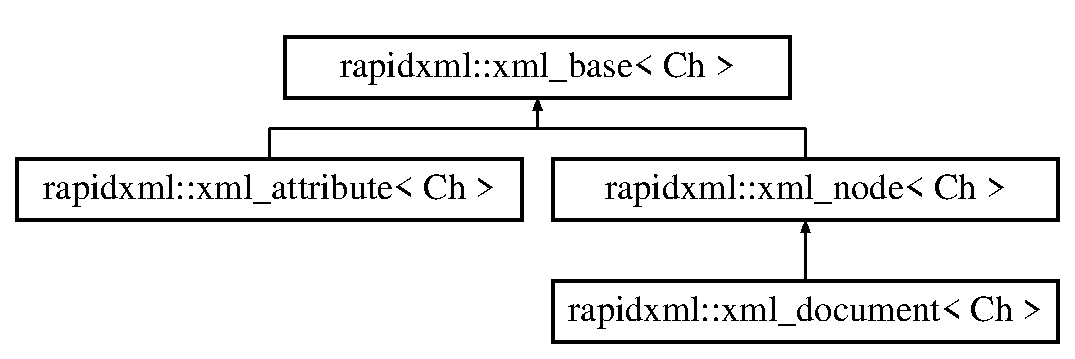
\includegraphics[height=3.000000cm]{classrapidxml_1_1xml__base}
\end{center}
\end{figure}
\subsection*{Public Member Functions}
\begin{DoxyCompactItemize}
\item 
Ch $\ast$ \hyperlink{classrapidxml_1_1xml__base_a9a09739310469995db078ebd0da3ed45}{name} () const 
\item 
std\+::size\+\_\+t \hyperlink{classrapidxml_1_1xml__base_a7e7f98b3d01e1eab8dc1ca69aad9af84}{name\+\_\+size} () const 
\item 
Ch $\ast$ \hyperlink{classrapidxml_1_1xml__base_adcdaccff61c665f039d9344e447b7445}{value} () const 
\item 
std\+::size\+\_\+t \hyperlink{classrapidxml_1_1xml__base_a9fcf201ed0915ac18dd43b0b5dcfaf32}{value\+\_\+size} () const 
\item 
void \hyperlink{classrapidxml_1_1xml__base_ae55060ae958c6e6465d6c8db852ec6ce}{name} (const Ch $\ast$name, std\+::size\+\_\+t size)
\item 
void \hyperlink{classrapidxml_1_1xml__base_a4611ddc82ac83a527c65606600eb2a0d}{name} (const Ch $\ast$name)
\item 
void \hyperlink{classrapidxml_1_1xml__base_a3b183c2db7022a6d30494dd2f0ac11e9}{value} (const Ch $\ast$value, std\+::size\+\_\+t size)
\item 
void \hyperlink{classrapidxml_1_1xml__base_a81e63ec4bfd2d7ef0a6c2ed49be6e623}{value} (const Ch $\ast$value)
\item 
\hyperlink{singletonrapidxml_1_1xml__node}{xml\+\_\+node}$<$ Ch $>$ $\ast$ \hyperlink{classrapidxml_1_1xml__base_a7f31ae930f93852830234db1ae59c4c4}{parent} () const 
\end{DoxyCompactItemize}
\subsection*{Static Protected Member Functions}
\begin{DoxyCompactItemize}
\item 
\hypertarget{classrapidxml_1_1xml__base_ad96ff6b1e41dab3ff60b9bc4df769a75}{static Ch $\ast$ {\bfseries nullstr} ()}\label{classrapidxml_1_1xml__base_ad96ff6b1e41dab3ff60b9bc4df769a75}

\end{DoxyCompactItemize}
\subsection*{Protected Attributes}
\begin{DoxyCompactItemize}
\item 
\hypertarget{classrapidxml_1_1xml__base_afd9851ed43e14619db0d7075ef8e9e8a}{Ch $\ast$ {\bfseries m\+\_\+name}}\label{classrapidxml_1_1xml__base_afd9851ed43e14619db0d7075ef8e9e8a}

\item 
\hypertarget{classrapidxml_1_1xml__base_a278a1ea63b0b70219b946cec47fa00ea}{Ch $\ast$ {\bfseries m\+\_\+value}}\label{classrapidxml_1_1xml__base_a278a1ea63b0b70219b946cec47fa00ea}

\item 
\hypertarget{classrapidxml_1_1xml__base_a5a8c76a7274b4180213796422c4df76f}{std\+::size\+\_\+t {\bfseries m\+\_\+name\+\_\+size}}\label{classrapidxml_1_1xml__base_a5a8c76a7274b4180213796422c4df76f}

\item 
\hypertarget{classrapidxml_1_1xml__base_aa3a49d8ceddb8a8d7edb773a2226b89c}{std\+::size\+\_\+t {\bfseries m\+\_\+value\+\_\+size}}\label{classrapidxml_1_1xml__base_aa3a49d8ceddb8a8d7edb773a2226b89c}

\item 
\hypertarget{classrapidxml_1_1xml__base_a90d5f660f078f66563fd7b2d8387ccb0}{\hyperlink{singletonrapidxml_1_1xml__node}{xml\+\_\+node}$<$ Ch $>$ $\ast$ {\bfseries m\+\_\+parent}}\label{classrapidxml_1_1xml__base_a90d5f660f078f66563fd7b2d8387ccb0}

\end{DoxyCompactItemize}


\subsection{Detailed Description}
\subsubsection*{template$<$class Ch = char$>$class rapidxml\+::xml\+\_\+base$<$ Ch $>$}

Base class for \hyperlink{singletonrapidxml_1_1xml__node}{xml\+\_\+node} and \hyperlink{singletonrapidxml_1_1xml__attribute}{xml\+\_\+attribute} implementing common functions\+: \hyperlink{classrapidxml_1_1xml__base_a9a09739310469995db078ebd0da3ed45}{name()}, \hyperlink{classrapidxml_1_1xml__base_a7e7f98b3d01e1eab8dc1ca69aad9af84}{name\+\_\+size()}, \hyperlink{classrapidxml_1_1xml__base_adcdaccff61c665f039d9344e447b7445}{value()}, \hyperlink{classrapidxml_1_1xml__base_a9fcf201ed0915ac18dd43b0b5dcfaf32}{value\+\_\+size()} and \hyperlink{classrapidxml_1_1xml__base_a7f31ae930f93852830234db1ae59c4c4}{parent()}. 
\begin{DoxyParams}{Parameters}
{\em Ch} & Character type to use \\
\hline
\end{DoxyParams}


\subsection{Member Function Documentation}
\hypertarget{classrapidxml_1_1xml__base_a9a09739310469995db078ebd0da3ed45}{\index{rapidxml\+::xml\+\_\+base@{rapidxml\+::xml\+\_\+base}!name@{name}}
\index{name@{name}!rapidxml\+::xml\+\_\+base@{rapidxml\+::xml\+\_\+base}}
\subsubsection[{name}]{\setlength{\rightskip}{0pt plus 5cm}template$<$class Ch  = char$>$ Ch$\ast$ {\bf rapidxml\+::xml\+\_\+base}$<$ Ch $>$\+::name (
\begin{DoxyParamCaption}
{}
\end{DoxyParamCaption}
) const\hspace{0.3cm}{\ttfamily [inline]}}}\label{classrapidxml_1_1xml__base_a9a09739310469995db078ebd0da3ed45}
Gets name of the node. Interpretation of name depends on type of node. Note that name will not be zero-\/terminated if rapidxml\+::parse\+\_\+no\+\_\+string\+\_\+terminators option was selected during parse. ~\newline
~\newline
 Use \hyperlink{classrapidxml_1_1xml__base_a7e7f98b3d01e1eab8dc1ca69aad9af84}{name\+\_\+size()} function to determine length of the name. \begin{DoxyReturn}{Returns}
Name of node, or empty string if node has no name. 
\end{DoxyReturn}
\hypertarget{classrapidxml_1_1xml__base_ae55060ae958c6e6465d6c8db852ec6ce}{\index{rapidxml\+::xml\+\_\+base@{rapidxml\+::xml\+\_\+base}!name@{name}}
\index{name@{name}!rapidxml\+::xml\+\_\+base@{rapidxml\+::xml\+\_\+base}}
\subsubsection[{name}]{\setlength{\rightskip}{0pt plus 5cm}template$<$class Ch  = char$>$ void {\bf rapidxml\+::xml\+\_\+base}$<$ Ch $>$\+::name (
\begin{DoxyParamCaption}
\item[{const Ch $\ast$}]{name, }
\item[{std\+::size\+\_\+t}]{size}
\end{DoxyParamCaption}
)\hspace{0.3cm}{\ttfamily [inline]}}}\label{classrapidxml_1_1xml__base_ae55060ae958c6e6465d6c8db852ec6ce}
Sets name of node to a non zero-\/terminated string. See ownership\+\_\+of\+\_\+strings. ~\newline
~\newline
 Note that node does not own its name or value, it only stores a pointer to it. It will not delete or otherwise free the pointer on destruction. It is reponsibility of the user to properly manage lifetime of the string. The easiest way to achieve it is to use \hyperlink{classrapidxml_1_1memory__pool}{memory\+\_\+pool} of the document to allocate the string -\/ on destruction of the document the string will be automatically freed. ~\newline
~\newline
 Size of name must be specified separately, because name does not have to be zero terminated. Use \hyperlink{classrapidxml_1_1xml__base_a4611ddc82ac83a527c65606600eb2a0d}{name(const Ch $\ast$)} function to have the length automatically calculated (string must be zero terminated). 
\begin{DoxyParams}{Parameters}
{\em name} & Name of node to set. Does not have to be zero terminated. \\
\hline
{\em size} & Size of name, in characters. This does not include zero terminator, if one is present. \\
\hline
\end{DoxyParams}
\hypertarget{classrapidxml_1_1xml__base_a4611ddc82ac83a527c65606600eb2a0d}{\index{rapidxml\+::xml\+\_\+base@{rapidxml\+::xml\+\_\+base}!name@{name}}
\index{name@{name}!rapidxml\+::xml\+\_\+base@{rapidxml\+::xml\+\_\+base}}
\subsubsection[{name}]{\setlength{\rightskip}{0pt plus 5cm}template$<$class Ch  = char$>$ void {\bf rapidxml\+::xml\+\_\+base}$<$ Ch $>$\+::name (
\begin{DoxyParamCaption}
\item[{const Ch $\ast$}]{name}
\end{DoxyParamCaption}
)\hspace{0.3cm}{\ttfamily [inline]}}}\label{classrapidxml_1_1xml__base_a4611ddc82ac83a527c65606600eb2a0d}
Sets name of node to a zero-\/terminated string. See also ownership\+\_\+of\+\_\+strings and \hyperlink{classrapidxml_1_1xml__base_ae55060ae958c6e6465d6c8db852ec6ce}{xml\+\_\+node\+::name(const Ch $\ast$, std\+::size\+\_\+t)}. 
\begin{DoxyParams}{Parameters}
{\em name} & Name of node to set. Must be zero terminated. \\
\hline
\end{DoxyParams}
\hypertarget{classrapidxml_1_1xml__base_a7e7f98b3d01e1eab8dc1ca69aad9af84}{\index{rapidxml\+::xml\+\_\+base@{rapidxml\+::xml\+\_\+base}!name\+\_\+size@{name\+\_\+size}}
\index{name\+\_\+size@{name\+\_\+size}!rapidxml\+::xml\+\_\+base@{rapidxml\+::xml\+\_\+base}}
\subsubsection[{name\+\_\+size}]{\setlength{\rightskip}{0pt plus 5cm}template$<$class Ch  = char$>$ std\+::size\+\_\+t {\bf rapidxml\+::xml\+\_\+base}$<$ Ch $>$\+::name\+\_\+size (
\begin{DoxyParamCaption}
{}
\end{DoxyParamCaption}
) const\hspace{0.3cm}{\ttfamily [inline]}}}\label{classrapidxml_1_1xml__base_a7e7f98b3d01e1eab8dc1ca69aad9af84}
Gets size of node name, not including terminator character. This function works correctly irrespective of whether name is or is not zero terminated. \begin{DoxyReturn}{Returns}
Size of node name, in characters. 
\end{DoxyReturn}
\hypertarget{classrapidxml_1_1xml__base_a7f31ae930f93852830234db1ae59c4c4}{\index{rapidxml\+::xml\+\_\+base@{rapidxml\+::xml\+\_\+base}!parent@{parent}}
\index{parent@{parent}!rapidxml\+::xml\+\_\+base@{rapidxml\+::xml\+\_\+base}}
\subsubsection[{parent}]{\setlength{\rightskip}{0pt plus 5cm}template$<$class Ch  = char$>$ {\bf xml\+\_\+node}$<$Ch$>$$\ast$ {\bf rapidxml\+::xml\+\_\+base}$<$ Ch $>$\+::parent (
\begin{DoxyParamCaption}
{}
\end{DoxyParamCaption}
) const\hspace{0.3cm}{\ttfamily [inline]}}}\label{classrapidxml_1_1xml__base_a7f31ae930f93852830234db1ae59c4c4}
Gets node parent. \begin{DoxyReturn}{Returns}
Pointer to parent node, or 0 if there is no parent. 
\end{DoxyReturn}
\hypertarget{classrapidxml_1_1xml__base_adcdaccff61c665f039d9344e447b7445}{\index{rapidxml\+::xml\+\_\+base@{rapidxml\+::xml\+\_\+base}!value@{value}}
\index{value@{value}!rapidxml\+::xml\+\_\+base@{rapidxml\+::xml\+\_\+base}}
\subsubsection[{value}]{\setlength{\rightskip}{0pt plus 5cm}template$<$class Ch  = char$>$ Ch$\ast$ {\bf rapidxml\+::xml\+\_\+base}$<$ Ch $>$\+::value (
\begin{DoxyParamCaption}
{}
\end{DoxyParamCaption}
) const\hspace{0.3cm}{\ttfamily [inline]}}}\label{classrapidxml_1_1xml__base_adcdaccff61c665f039d9344e447b7445}
Gets value of node. Interpretation of value depends on type of node. Note that value will not be zero-\/terminated if rapidxml\+::parse\+\_\+no\+\_\+string\+\_\+terminators option was selected during parse. ~\newline
~\newline
 Use \hyperlink{classrapidxml_1_1xml__base_a9fcf201ed0915ac18dd43b0b5dcfaf32}{value\+\_\+size()} function to determine length of the value. \begin{DoxyReturn}{Returns}
Value of node, or empty string if node has no value. 
\end{DoxyReturn}
\hypertarget{classrapidxml_1_1xml__base_a3b183c2db7022a6d30494dd2f0ac11e9}{\index{rapidxml\+::xml\+\_\+base@{rapidxml\+::xml\+\_\+base}!value@{value}}
\index{value@{value}!rapidxml\+::xml\+\_\+base@{rapidxml\+::xml\+\_\+base}}
\subsubsection[{value}]{\setlength{\rightskip}{0pt plus 5cm}template$<$class Ch  = char$>$ void {\bf rapidxml\+::xml\+\_\+base}$<$ Ch $>$\+::value (
\begin{DoxyParamCaption}
\item[{const Ch $\ast$}]{value, }
\item[{std\+::size\+\_\+t}]{size}
\end{DoxyParamCaption}
)\hspace{0.3cm}{\ttfamily [inline]}}}\label{classrapidxml_1_1xml__base_a3b183c2db7022a6d30494dd2f0ac11e9}
Sets value of node to a non zero-\/terminated string. See ownership\+\_\+of\+\_\+strings. ~\newline
~\newline
 Note that node does not own its name or value, it only stores a pointer to it. It will not delete or otherwise free the pointer on destruction. It is reponsibility of the user to properly manage lifetime of the string. The easiest way to achieve it is to use \hyperlink{classrapidxml_1_1memory__pool}{memory\+\_\+pool} of the document to allocate the string -\/ on destruction of the document the string will be automatically freed. ~\newline
~\newline
 Size of value must be specified separately, because it does not have to be zero terminated. Use \hyperlink{classrapidxml_1_1xml__base_a81e63ec4bfd2d7ef0a6c2ed49be6e623}{value(const Ch $\ast$)} function to have the length automatically calculated (string must be zero terminated). ~\newline
~\newline
 If an element has a child node of type node\+\_\+data, it will take precedence over element value when printing. If you want to manipulate data of elements using values, use parser flag rapidxml\+::parse\+\_\+no\+\_\+data\+\_\+nodes to prevent creation of data nodes by the parser. 
\begin{DoxyParams}{Parameters}
{\em value} & value of node to set. Does not have to be zero terminated. \\
\hline
{\em size} & Size of value, in characters. This does not include zero terminator, if one is present. \\
\hline
\end{DoxyParams}
\hypertarget{classrapidxml_1_1xml__base_a81e63ec4bfd2d7ef0a6c2ed49be6e623}{\index{rapidxml\+::xml\+\_\+base@{rapidxml\+::xml\+\_\+base}!value@{value}}
\index{value@{value}!rapidxml\+::xml\+\_\+base@{rapidxml\+::xml\+\_\+base}}
\subsubsection[{value}]{\setlength{\rightskip}{0pt plus 5cm}template$<$class Ch  = char$>$ void {\bf rapidxml\+::xml\+\_\+base}$<$ Ch $>$\+::value (
\begin{DoxyParamCaption}
\item[{const Ch $\ast$}]{value}
\end{DoxyParamCaption}
)\hspace{0.3cm}{\ttfamily [inline]}}}\label{classrapidxml_1_1xml__base_a81e63ec4bfd2d7ef0a6c2ed49be6e623}
Sets value of node to a zero-\/terminated string. See also ownership\+\_\+of\+\_\+strings and \hyperlink{classrapidxml_1_1xml__base_a3b183c2db7022a6d30494dd2f0ac11e9}{xml\+\_\+node\+::value(const Ch $\ast$, std\+::size\+\_\+t)}. 
\begin{DoxyParams}{Parameters}
{\em value} & Vame of node to set. Must be zero terminated. \\
\hline
\end{DoxyParams}
\hypertarget{classrapidxml_1_1xml__base_a9fcf201ed0915ac18dd43b0b5dcfaf32}{\index{rapidxml\+::xml\+\_\+base@{rapidxml\+::xml\+\_\+base}!value\+\_\+size@{value\+\_\+size}}
\index{value\+\_\+size@{value\+\_\+size}!rapidxml\+::xml\+\_\+base@{rapidxml\+::xml\+\_\+base}}
\subsubsection[{value\+\_\+size}]{\setlength{\rightskip}{0pt plus 5cm}template$<$class Ch  = char$>$ std\+::size\+\_\+t {\bf rapidxml\+::xml\+\_\+base}$<$ Ch $>$\+::value\+\_\+size (
\begin{DoxyParamCaption}
{}
\end{DoxyParamCaption}
) const\hspace{0.3cm}{\ttfamily [inline]}}}\label{classrapidxml_1_1xml__base_a9fcf201ed0915ac18dd43b0b5dcfaf32}
Gets size of node value, not including terminator character. This function works correctly irrespective of whether value is or is not zero terminated. \begin{DoxyReturn}{Returns}
Size of node value, in characters. 
\end{DoxyReturn}


The documentation for this class was generated from the following file\+:\begin{DoxyCompactItemize}
\item 
\hyperlink{rapidxml_8hpp}{rapidxml.\+hpp}\end{DoxyCompactItemize}

\hypertarget{singletonrapidxml_1_1xml__document}{\section{rapidxml\+:\+:xml\+\_\+document$<$ Ch $>$ Class Template Reference}
\label{singletonrapidxml_1_1xml__document}\index{rapidxml\+::xml\+\_\+document$<$ Ch $>$@{rapidxml\+::xml\+\_\+document$<$ Ch $>$}}
}


{\ttfamily \#include $<$rapidxml.\+hpp$>$}

Inheritance diagram for rapidxml\+:\+:xml\+\_\+document$<$ Ch $>$\+:\begin{figure}[H]
\begin{center}
\leavevmode
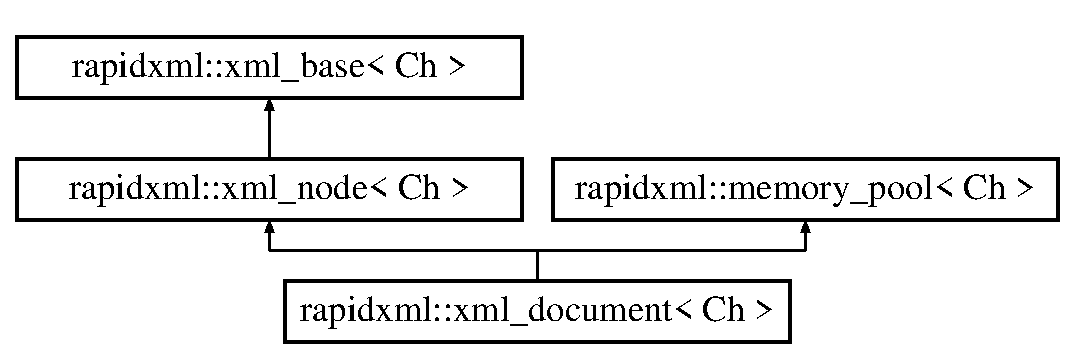
\includegraphics[height=3.000000cm]{singletonrapidxml_1_1xml__document}
\end{center}
\end{figure}
\subsection*{Public Member Functions}
\begin{DoxyCompactItemize}
\item 
\hypertarget{singletonrapidxml_1_1xml__document_aae8841b15085ba8f32ff46587ace28f5}{\hyperlink{singletonrapidxml_1_1xml__document_aae8841b15085ba8f32ff46587ace28f5}{xml\+\_\+document} ()}\label{singletonrapidxml_1_1xml__document_aae8841b15085ba8f32ff46587ace28f5}

\begin{DoxyCompactList}\small\item\em Constructs empty X\+M\+L document. \end{DoxyCompactList}\item 
{\footnotesize template$<$int Flags$>$ }\\void \hyperlink{singletonrapidxml_1_1xml__document_ac6e73ff9ac323bf5a370c38feb03a6b1}{parse} (Ch $\ast$text)
\item 
void \hyperlink{singletonrapidxml_1_1xml__document_a826929ff54242532198701f19ff5f83f}{clear} ()
\end{DoxyCompactItemize}
\subsection*{Additional Inherited Members}


\subsection{Detailed Description}
\subsubsection*{template$<$class Ch = char$>$class rapidxml\+::xml\+\_\+document$<$ Ch $>$}

This class represents root of the D\+O\+M hierarchy. It is also an \hyperlink{singletonrapidxml_1_1xml__node}{xml\+\_\+node} and a \hyperlink{classrapidxml_1_1memory__pool}{memory\+\_\+pool} through public inheritance. Use \hyperlink{singletonrapidxml_1_1xml__document_ac6e73ff9ac323bf5a370c38feb03a6b1}{parse()} function to build a D\+O\+M tree from a zero-\/terminated X\+M\+L text string. \hyperlink{singletonrapidxml_1_1xml__document_ac6e73ff9ac323bf5a370c38feb03a6b1}{parse()} function allocates memory for nodes and attributes by using functions of \hyperlink{singletonrapidxml_1_1xml__document}{xml\+\_\+document}, which are inherited from \hyperlink{classrapidxml_1_1memory__pool}{memory\+\_\+pool}. To access root node of the document, use the document itself, as if it was an \hyperlink{singletonrapidxml_1_1xml__node}{xml\+\_\+node}. 
\begin{DoxyParams}{Parameters}
{\em Ch} & Character type to use. \\
\hline
\end{DoxyParams}


\subsection{Member Function Documentation}
\hypertarget{singletonrapidxml_1_1xml__document_a826929ff54242532198701f19ff5f83f}{\index{rapidxml\+::xml\+\_\+document@{rapidxml\+::xml\+\_\+document}!clear@{clear}}
\index{clear@{clear}!rapidxml\+::xml\+\_\+document@{rapidxml\+::xml\+\_\+document}}
\subsubsection[{clear}]{\setlength{\rightskip}{0pt plus 5cm}template$<$class Ch  = char$>$ void {\bf rapidxml\+::xml\+\_\+document}$<$ Ch $>$\+::clear (
\begin{DoxyParamCaption}
{}
\end{DoxyParamCaption}
)\hspace{0.3cm}{\ttfamily [inline]}}}\label{singletonrapidxml_1_1xml__document_a826929ff54242532198701f19ff5f83f}
Clears the document by deleting all nodes and clearing the memory pool. All nodes owned by document pool are destroyed. \hypertarget{singletonrapidxml_1_1xml__document_ac6e73ff9ac323bf5a370c38feb03a6b1}{\index{rapidxml\+::xml\+\_\+document@{rapidxml\+::xml\+\_\+document}!parse@{parse}}
\index{parse@{parse}!rapidxml\+::xml\+\_\+document@{rapidxml\+::xml\+\_\+document}}
\subsubsection[{parse}]{\setlength{\rightskip}{0pt plus 5cm}template$<$class Ch  = char$>$ template$<$int Flags$>$ void {\bf rapidxml\+::xml\+\_\+document}$<$ Ch $>$\+::parse (
\begin{DoxyParamCaption}
\item[{Ch $\ast$}]{text}
\end{DoxyParamCaption}
)\hspace{0.3cm}{\ttfamily [inline]}}}\label{singletonrapidxml_1_1xml__document_ac6e73ff9ac323bf5a370c38feb03a6b1}
Parses zero-\/terminated X\+M\+L string according to given flags. Passed string will be modified by the parser, unless rapidxml\+::parse\+\_\+non\+\_\+destructive flag is used. The string must persist for the lifetime of the document. In case of error, \hyperlink{classrapidxml_1_1parse__error}{rapidxml\+::parse\+\_\+error} exception will be thrown. ~\newline
~\newline
 If you want to parse contents of a file, you must first load the file into the memory, and pass pointer to its beginning. Make sure that data is zero-\/terminated. ~\newline
~\newline
 Document can be parsed into multiple times. Each new call to parse removes previous nodes and attributes (if any), but does not clear memory pool. 
\begin{DoxyParams}{Parameters}
{\em text} & X\+M\+L data to parse; pointer is non-\/const to denote fact that this data may be modified by the parser. \\
\hline
\end{DoxyParams}


The documentation for this class was generated from the following file\+:\begin{DoxyCompactItemize}
\item 
\hyperlink{rapidxml_8hpp}{rapidxml.\+hpp}\end{DoxyCompactItemize}

\hypertarget{singletonrapidxml_1_1xml__node}{\section{rapidxml\+:\+:xml\+\_\+node$<$ Ch $>$ Class Template Reference}
\label{singletonrapidxml_1_1xml__node}\index{rapidxml\+::xml\+\_\+node$<$ Ch $>$@{rapidxml\+::xml\+\_\+node$<$ Ch $>$}}
}


{\ttfamily \#include $<$rapidxml.\+hpp$>$}

Inheritance diagram for rapidxml\+:\+:xml\+\_\+node$<$ Ch $>$\+:\begin{figure}[H]
\begin{center}
\leavevmode
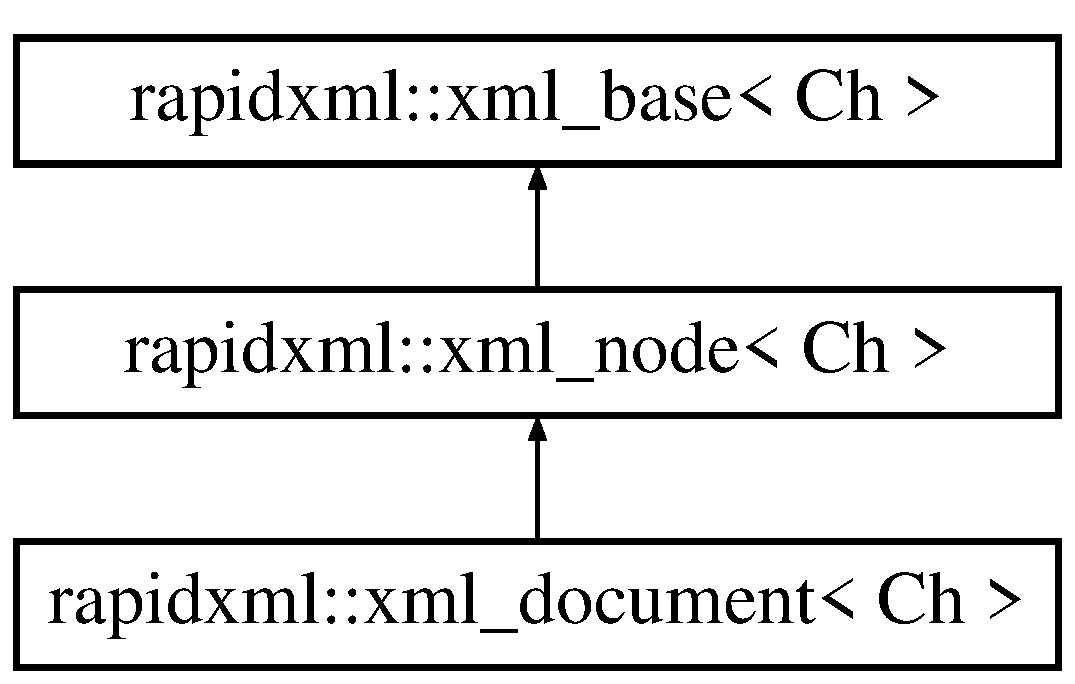
\includegraphics[height=3.000000cm]{singletonrapidxml_1_1xml__node}
\end{center}
\end{figure}
\subsection*{Public Member Functions}
\begin{DoxyCompactItemize}
\item 
\hyperlink{singletonrapidxml_1_1xml__node_a8bd9019960b90605a45998b661fb1b0e}{xml\+\_\+node} (node\+\_\+type \hyperlink{singletonrapidxml_1_1xml__node_a2c6a4315b98bcfa2e04fed3fa1b22c36}{type})
\item 
node\+\_\+type \hyperlink{singletonrapidxml_1_1xml__node_a2c6a4315b98bcfa2e04fed3fa1b22c36}{type} () const 
\item 
\hyperlink{singletonrapidxml_1_1xml__document}{xml\+\_\+document}$<$ Ch $>$ $\ast$ \hyperlink{singletonrapidxml_1_1xml__node_adb6ad21a4590cf13d4a6a5036e3cdbbc}{document} () const 
\item 
\hyperlink{singletonrapidxml_1_1xml__node}{xml\+\_\+node}$<$ Ch $>$ $\ast$ \hyperlink{singletonrapidxml_1_1xml__node_a2dedeb4e04bb35e06a9a7bddf6ba652d}{first\+\_\+node} (const Ch $\ast$\hyperlink{classrapidxml_1_1xml__base_a9a09739310469995db078ebd0da3ed45}{name}=0, std\+::size\+\_\+t \hyperlink{classrapidxml_1_1xml__base_a7e7f98b3d01e1eab8dc1ca69aad9af84}{name\+\_\+size}=0, bool case\+\_\+sensitive=true) const 
\item 
\hyperlink{singletonrapidxml_1_1xml__node}{xml\+\_\+node}$<$ Ch $>$ $\ast$ \hyperlink{singletonrapidxml_1_1xml__node_a2ace550c18cf10da6303773972d7157f}{last\+\_\+node} (const Ch $\ast$\hyperlink{classrapidxml_1_1xml__base_a9a09739310469995db078ebd0da3ed45}{name}=0, std\+::size\+\_\+t \hyperlink{classrapidxml_1_1xml__base_a7e7f98b3d01e1eab8dc1ca69aad9af84}{name\+\_\+size}=0, bool case\+\_\+sensitive=true) const 
\item 
\hyperlink{singletonrapidxml_1_1xml__node}{xml\+\_\+node}$<$ Ch $>$ $\ast$ \hyperlink{singletonrapidxml_1_1xml__node_a001ece4e227eebbd6ad0ec7dacf1c00b}{previous\+\_\+sibling} (const Ch $\ast$\hyperlink{classrapidxml_1_1xml__base_a9a09739310469995db078ebd0da3ed45}{name}=0, std\+::size\+\_\+t \hyperlink{classrapidxml_1_1xml__base_a7e7f98b3d01e1eab8dc1ca69aad9af84}{name\+\_\+size}=0, bool case\+\_\+sensitive=true) const 
\item 
\hyperlink{singletonrapidxml_1_1xml__node}{xml\+\_\+node}$<$ Ch $>$ $\ast$ \hyperlink{singletonrapidxml_1_1xml__node_ac59af4dd5f0ec715753e42467dff6aed}{next\+\_\+sibling} (const Ch $\ast$\hyperlink{classrapidxml_1_1xml__base_a9a09739310469995db078ebd0da3ed45}{name}=0, std\+::size\+\_\+t \hyperlink{classrapidxml_1_1xml__base_a7e7f98b3d01e1eab8dc1ca69aad9af84}{name\+\_\+size}=0, bool case\+\_\+sensitive=true) const 
\item 
\hyperlink{singletonrapidxml_1_1xml__attribute}{xml\+\_\+attribute}$<$ Ch $>$ $\ast$ \hyperlink{singletonrapidxml_1_1xml__node_ae426802be58114ffc41bf30ac6b8c37d}{first\+\_\+attribute} (const Ch $\ast$\hyperlink{classrapidxml_1_1xml__base_a9a09739310469995db078ebd0da3ed45}{name}=0, std\+::size\+\_\+t \hyperlink{classrapidxml_1_1xml__base_a7e7f98b3d01e1eab8dc1ca69aad9af84}{name\+\_\+size}=0, bool case\+\_\+sensitive=true) const 
\item 
\hyperlink{singletonrapidxml_1_1xml__attribute}{xml\+\_\+attribute}$<$ Ch $>$ $\ast$ \hyperlink{singletonrapidxml_1_1xml__node_a50c03f2db3fa51f27a73d86ec29a49d3}{last\+\_\+attribute} (const Ch $\ast$\hyperlink{classrapidxml_1_1xml__base_a9a09739310469995db078ebd0da3ed45}{name}=0, std\+::size\+\_\+t \hyperlink{classrapidxml_1_1xml__base_a7e7f98b3d01e1eab8dc1ca69aad9af84}{name\+\_\+size}=0, bool case\+\_\+sensitive=true) const 
\item 
void \hyperlink{singletonrapidxml_1_1xml__node_a499bbc9300c1b06821d5c08b24164c68}{type} (node\+\_\+type type)
\item 
void \hyperlink{singletonrapidxml_1_1xml__node_ae86e92908c3eab40bbed8216e4f3f3cb}{prepend\+\_\+node} (\hyperlink{singletonrapidxml_1_1xml__node}{xml\+\_\+node}$<$ Ch $>$ $\ast$child)
\item 
void \hyperlink{singletonrapidxml_1_1xml__node_a8696d098ecc9c4d2a646b43e91d58e31}{append\+\_\+node} (\hyperlink{singletonrapidxml_1_1xml__node}{xml\+\_\+node}$<$ Ch $>$ $\ast$child)
\item 
void \hyperlink{singletonrapidxml_1_1xml__node_a666880f42a7e486d78cc45ed51c7c46d}{insert\+\_\+node} (\hyperlink{singletonrapidxml_1_1xml__node}{xml\+\_\+node}$<$ Ch $>$ $\ast$where, \hyperlink{singletonrapidxml_1_1xml__node}{xml\+\_\+node}$<$ Ch $>$ $\ast$child)
\item 
void \hyperlink{singletonrapidxml_1_1xml__node_a62bf7b276cf7a651a3337f5e0a0ef6ac}{remove\+\_\+first\+\_\+node} ()
\item 
void \hyperlink{singletonrapidxml_1_1xml__node_a9182512e948ec451a83f116cce7c7674}{remove\+\_\+last\+\_\+node} ()
\item 
\hypertarget{singletonrapidxml_1_1xml__node_a98289923eb9e8889418a9eb0207ea35c}{void \hyperlink{singletonrapidxml_1_1xml__node_a98289923eb9e8889418a9eb0207ea35c}{remove\+\_\+node} (\hyperlink{singletonrapidxml_1_1xml__node}{xml\+\_\+node}$<$ Ch $>$ $\ast$where)}\label{singletonrapidxml_1_1xml__node_a98289923eb9e8889418a9eb0207ea35c}

\begin{DoxyCompactList}\small\item\em Removes specified child from the node. \end{DoxyCompactList}\item 
\hypertarget{singletonrapidxml_1_1xml__node_a95735358b079ae0adcfbbac69aa1fbc3}{void \hyperlink{singletonrapidxml_1_1xml__node_a95735358b079ae0adcfbbac69aa1fbc3}{remove\+\_\+all\+\_\+nodes} ()}\label{singletonrapidxml_1_1xml__node_a95735358b079ae0adcfbbac69aa1fbc3}

\begin{DoxyCompactList}\small\item\em Removes all child nodes (but not attributes). \end{DoxyCompactList}\item 
void \hyperlink{singletonrapidxml_1_1xml__node_a8b62ee76489faf8e2d1210869d547684}{prepend\+\_\+attribute} (\hyperlink{singletonrapidxml_1_1xml__attribute}{xml\+\_\+attribute}$<$ Ch $>$ $\ast$attribute)
\item 
void \hyperlink{singletonrapidxml_1_1xml__node_a33ce3386f8c42dd4db658b75cbb6e6c4}{append\+\_\+attribute} (\hyperlink{singletonrapidxml_1_1xml__attribute}{xml\+\_\+attribute}$<$ Ch $>$ $\ast$attribute)
\item 
void \hyperlink{singletonrapidxml_1_1xml__node_a9fe659cdf4a5b3bbf5e8ffc98db5a84f}{insert\+\_\+attribute} (\hyperlink{singletonrapidxml_1_1xml__attribute}{xml\+\_\+attribute}$<$ Ch $>$ $\ast$where, \hyperlink{singletonrapidxml_1_1xml__attribute}{xml\+\_\+attribute}$<$ Ch $>$ $\ast$attribute)
\item 
void \hyperlink{singletonrapidxml_1_1xml__node_aa95192d2a165cca16c551ed2a2a06aec}{remove\+\_\+first\+\_\+attribute} ()
\item 
void \hyperlink{singletonrapidxml_1_1xml__node_a1781a2cbedc9a51d609ad5b528125635}{remove\+\_\+last\+\_\+attribute} ()
\item 
void \hyperlink{singletonrapidxml_1_1xml__node_a6f97b1b4f46a94a4587915df3c0c6b57}{remove\+\_\+attribute} (\hyperlink{singletonrapidxml_1_1xml__attribute}{xml\+\_\+attribute}$<$ Ch $>$ $\ast$where)
\item 
\hypertarget{singletonrapidxml_1_1xml__node_aa8d5d9484aa1eb5ff1841a073c84c1aa}{void \hyperlink{singletonrapidxml_1_1xml__node_aa8d5d9484aa1eb5ff1841a073c84c1aa}{remove\+\_\+all\+\_\+attributes} ()}\label{singletonrapidxml_1_1xml__node_aa8d5d9484aa1eb5ff1841a073c84c1aa}

\begin{DoxyCompactList}\small\item\em Removes all attributes of node. \end{DoxyCompactList}\end{DoxyCompactItemize}
\subsection*{Additional Inherited Members}


\subsection{Detailed Description}
\subsubsection*{template$<$class Ch = char$>$class rapidxml\+::xml\+\_\+node$<$ Ch $>$}

Class representing a node of X\+M\+L document. Each node may have associated name and value strings, which are available through \hyperlink{classrapidxml_1_1xml__base_a9a09739310469995db078ebd0da3ed45}{name()} and \hyperlink{classrapidxml_1_1xml__base_adcdaccff61c665f039d9344e447b7445}{value()} functions. Interpretation of name and value depends on type of the node. Type of node can be determined by using \hyperlink{singletonrapidxml_1_1xml__node_a2c6a4315b98bcfa2e04fed3fa1b22c36}{type()} function. ~\newline
~\newline
 Note that after parse, both name and value of node, if any, will point interior of source text used for parsing. Thus, this text must persist in the memory for the lifetime of node. 
\begin{DoxyParams}{Parameters}
{\em Ch} & Character type to use. \\
\hline
\end{DoxyParams}


\subsection{Constructor \& Destructor Documentation}
\hypertarget{singletonrapidxml_1_1xml__node_a8bd9019960b90605a45998b661fb1b0e}{\index{rapidxml\+::xml\+\_\+node@{rapidxml\+::xml\+\_\+node}!xml\+\_\+node@{xml\+\_\+node}}
\index{xml\+\_\+node@{xml\+\_\+node}!rapidxml\+::xml\+\_\+node@{rapidxml\+::xml\+\_\+node}}
\subsubsection[{xml\+\_\+node}]{\setlength{\rightskip}{0pt plus 5cm}template$<$class Ch = char$>$ {\bf rapidxml\+::xml\+\_\+node}$<$ Ch $>$\+::{\bf xml\+\_\+node} (
\begin{DoxyParamCaption}
\item[{node\+\_\+type}]{type}
\end{DoxyParamCaption}
)\hspace{0.3cm}{\ttfamily [inline]}}}\label{singletonrapidxml_1_1xml__node_a8bd9019960b90605a45998b661fb1b0e}
Constructs an empty node with the specified type. Consider using \hyperlink{classrapidxml_1_1memory__pool}{memory\+\_\+pool} of appropriate document to allocate nodes manually. 
\begin{DoxyParams}{Parameters}
{\em type} & Type of node to construct. \\
\hline
\end{DoxyParams}


\subsection{Member Function Documentation}
\hypertarget{singletonrapidxml_1_1xml__node_a33ce3386f8c42dd4db658b75cbb6e6c4}{\index{rapidxml\+::xml\+\_\+node@{rapidxml\+::xml\+\_\+node}!append\+\_\+attribute@{append\+\_\+attribute}}
\index{append\+\_\+attribute@{append\+\_\+attribute}!rapidxml\+::xml\+\_\+node@{rapidxml\+::xml\+\_\+node}}
\subsubsection[{append\+\_\+attribute}]{\setlength{\rightskip}{0pt plus 5cm}template$<$class Ch = char$>$ void {\bf rapidxml\+::xml\+\_\+node}$<$ Ch $>$\+::append\+\_\+attribute (
\begin{DoxyParamCaption}
\item[{{\bf xml\+\_\+attribute}$<$ Ch $>$ $\ast$}]{attribute}
\end{DoxyParamCaption}
)\hspace{0.3cm}{\ttfamily [inline]}}}\label{singletonrapidxml_1_1xml__node_a33ce3386f8c42dd4db658b75cbb6e6c4}
Appends a new attribute to the node. 
\begin{DoxyParams}{Parameters}
{\em attribute} & Attribute to append. \\
\hline
\end{DoxyParams}
\hypertarget{singletonrapidxml_1_1xml__node_a8696d098ecc9c4d2a646b43e91d58e31}{\index{rapidxml\+::xml\+\_\+node@{rapidxml\+::xml\+\_\+node}!append\+\_\+node@{append\+\_\+node}}
\index{append\+\_\+node@{append\+\_\+node}!rapidxml\+::xml\+\_\+node@{rapidxml\+::xml\+\_\+node}}
\subsubsection[{append\+\_\+node}]{\setlength{\rightskip}{0pt plus 5cm}template$<$class Ch = char$>$ void {\bf rapidxml\+::xml\+\_\+node}$<$ Ch $>$\+::append\+\_\+node (
\begin{DoxyParamCaption}
\item[{{\bf xml\+\_\+node}$<$ Ch $>$ $\ast$}]{child}
\end{DoxyParamCaption}
)\hspace{0.3cm}{\ttfamily [inline]}}}\label{singletonrapidxml_1_1xml__node_a8696d098ecc9c4d2a646b43e91d58e31}
Appends a new child node. The appended child becomes the last child. 
\begin{DoxyParams}{Parameters}
{\em child} & Node to append. \\
\hline
\end{DoxyParams}
\hypertarget{singletonrapidxml_1_1xml__node_adb6ad21a4590cf13d4a6a5036e3cdbbc}{\index{rapidxml\+::xml\+\_\+node@{rapidxml\+::xml\+\_\+node}!document@{document}}
\index{document@{document}!rapidxml\+::xml\+\_\+node@{rapidxml\+::xml\+\_\+node}}
\subsubsection[{document}]{\setlength{\rightskip}{0pt plus 5cm}template$<$class Ch = char$>$ {\bf xml\+\_\+document}$<$Ch$>$$\ast$ {\bf rapidxml\+::xml\+\_\+node}$<$ Ch $>$\+::document (
\begin{DoxyParamCaption}
{}
\end{DoxyParamCaption}
) const\hspace{0.3cm}{\ttfamily [inline]}}}\label{singletonrapidxml_1_1xml__node_adb6ad21a4590cf13d4a6a5036e3cdbbc}
Gets document of which node is a child. \begin{DoxyReturn}{Returns}
Pointer to document that contains this node, or 0 if there is no parent document. 
\end{DoxyReturn}
\hypertarget{singletonrapidxml_1_1xml__node_ae426802be58114ffc41bf30ac6b8c37d}{\index{rapidxml\+::xml\+\_\+node@{rapidxml\+::xml\+\_\+node}!first\+\_\+attribute@{first\+\_\+attribute}}
\index{first\+\_\+attribute@{first\+\_\+attribute}!rapidxml\+::xml\+\_\+node@{rapidxml\+::xml\+\_\+node}}
\subsubsection[{first\+\_\+attribute}]{\setlength{\rightskip}{0pt plus 5cm}template$<$class Ch = char$>$ {\bf xml\+\_\+attribute}$<$Ch$>$$\ast$ {\bf rapidxml\+::xml\+\_\+node}$<$ Ch $>$\+::first\+\_\+attribute (
\begin{DoxyParamCaption}
\item[{const Ch $\ast$}]{name = {\ttfamily 0}, }
\item[{std\+::size\+\_\+t}]{name\+\_\+size = {\ttfamily 0}, }
\item[{bool}]{case\+\_\+sensitive = {\ttfamily true}}
\end{DoxyParamCaption}
) const\hspace{0.3cm}{\ttfamily [inline]}}}\label{singletonrapidxml_1_1xml__node_ae426802be58114ffc41bf30ac6b8c37d}
Gets first attribute of node, optionally matching attribute name. 
\begin{DoxyParams}{Parameters}
{\em name} & Name of attribute to find, or 0 to return first attribute regardless of its name; this string doesn't have to be zero-\/terminated if name\+\_\+size is non-\/zero \\
\hline
{\em name\+\_\+size} & Size of name, in characters, or 0 to have size calculated automatically from string \\
\hline
{\em case\+\_\+sensitive} & Should name comparison be case-\/sensitive; non case-\/sensitive comparison works properly only for A\+S\+C\+I\+I characters \\
\hline
\end{DoxyParams}
\begin{DoxyReturn}{Returns}
Pointer to found attribute, or 0 if not found. 
\end{DoxyReturn}
\hypertarget{singletonrapidxml_1_1xml__node_a2dedeb4e04bb35e06a9a7bddf6ba652d}{\index{rapidxml\+::xml\+\_\+node@{rapidxml\+::xml\+\_\+node}!first\+\_\+node@{first\+\_\+node}}
\index{first\+\_\+node@{first\+\_\+node}!rapidxml\+::xml\+\_\+node@{rapidxml\+::xml\+\_\+node}}
\subsubsection[{first\+\_\+node}]{\setlength{\rightskip}{0pt plus 5cm}template$<$class Ch = char$>$ {\bf xml\+\_\+node}$<$Ch$>$$\ast$ {\bf rapidxml\+::xml\+\_\+node}$<$ Ch $>$\+::first\+\_\+node (
\begin{DoxyParamCaption}
\item[{const Ch $\ast$}]{name = {\ttfamily 0}, }
\item[{std\+::size\+\_\+t}]{name\+\_\+size = {\ttfamily 0}, }
\item[{bool}]{case\+\_\+sensitive = {\ttfamily true}}
\end{DoxyParamCaption}
) const\hspace{0.3cm}{\ttfamily [inline]}}}\label{singletonrapidxml_1_1xml__node_a2dedeb4e04bb35e06a9a7bddf6ba652d}
Gets first child node, optionally matching node name. 
\begin{DoxyParams}{Parameters}
{\em name} & Name of child to find, or 0 to return first child regardless of its name; this string doesn't have to be zero-\/terminated if name\+\_\+size is non-\/zero \\
\hline
{\em name\+\_\+size} & Size of name, in characters, or 0 to have size calculated automatically from string \\
\hline
{\em case\+\_\+sensitive} & Should name comparison be case-\/sensitive; non case-\/sensitive comparison works properly only for A\+S\+C\+I\+I characters \\
\hline
\end{DoxyParams}
\begin{DoxyReturn}{Returns}
Pointer to found child, or 0 if not found. 
\end{DoxyReturn}
\hypertarget{singletonrapidxml_1_1xml__node_a9fe659cdf4a5b3bbf5e8ffc98db5a84f}{\index{rapidxml\+::xml\+\_\+node@{rapidxml\+::xml\+\_\+node}!insert\+\_\+attribute@{insert\+\_\+attribute}}
\index{insert\+\_\+attribute@{insert\+\_\+attribute}!rapidxml\+::xml\+\_\+node@{rapidxml\+::xml\+\_\+node}}
\subsubsection[{insert\+\_\+attribute}]{\setlength{\rightskip}{0pt plus 5cm}template$<$class Ch = char$>$ void {\bf rapidxml\+::xml\+\_\+node}$<$ Ch $>$\+::insert\+\_\+attribute (
\begin{DoxyParamCaption}
\item[{{\bf xml\+\_\+attribute}$<$ Ch $>$ $\ast$}]{where, }
\item[{{\bf xml\+\_\+attribute}$<$ Ch $>$ $\ast$}]{attribute}
\end{DoxyParamCaption}
)\hspace{0.3cm}{\ttfamily [inline]}}}\label{singletonrapidxml_1_1xml__node_a9fe659cdf4a5b3bbf5e8ffc98db5a84f}
Inserts a new attribute at specified place inside the node. All attributes after and including the specified attribute are moved one position back. 
\begin{DoxyParams}{Parameters}
{\em where} & Place where to insert the attribute, or 0 to insert at the back. \\
\hline
{\em attribute} & Attribute to insert. \\
\hline
\end{DoxyParams}
\hypertarget{singletonrapidxml_1_1xml__node_a666880f42a7e486d78cc45ed51c7c46d}{\index{rapidxml\+::xml\+\_\+node@{rapidxml\+::xml\+\_\+node}!insert\+\_\+node@{insert\+\_\+node}}
\index{insert\+\_\+node@{insert\+\_\+node}!rapidxml\+::xml\+\_\+node@{rapidxml\+::xml\+\_\+node}}
\subsubsection[{insert\+\_\+node}]{\setlength{\rightskip}{0pt plus 5cm}template$<$class Ch = char$>$ void {\bf rapidxml\+::xml\+\_\+node}$<$ Ch $>$\+::insert\+\_\+node (
\begin{DoxyParamCaption}
\item[{{\bf xml\+\_\+node}$<$ Ch $>$ $\ast$}]{where, }
\item[{{\bf xml\+\_\+node}$<$ Ch $>$ $\ast$}]{child}
\end{DoxyParamCaption}
)\hspace{0.3cm}{\ttfamily [inline]}}}\label{singletonrapidxml_1_1xml__node_a666880f42a7e486d78cc45ed51c7c46d}
Inserts a new child node at specified place inside the node. All children after and including the specified node are moved one position back. 
\begin{DoxyParams}{Parameters}
{\em where} & Place where to insert the child, or 0 to insert at the back. \\
\hline
{\em child} & Node to insert. \\
\hline
\end{DoxyParams}
\hypertarget{singletonrapidxml_1_1xml__node_a50c03f2db3fa51f27a73d86ec29a49d3}{\index{rapidxml\+::xml\+\_\+node@{rapidxml\+::xml\+\_\+node}!last\+\_\+attribute@{last\+\_\+attribute}}
\index{last\+\_\+attribute@{last\+\_\+attribute}!rapidxml\+::xml\+\_\+node@{rapidxml\+::xml\+\_\+node}}
\subsubsection[{last\+\_\+attribute}]{\setlength{\rightskip}{0pt plus 5cm}template$<$class Ch = char$>$ {\bf xml\+\_\+attribute}$<$Ch$>$$\ast$ {\bf rapidxml\+::xml\+\_\+node}$<$ Ch $>$\+::last\+\_\+attribute (
\begin{DoxyParamCaption}
\item[{const Ch $\ast$}]{name = {\ttfamily 0}, }
\item[{std\+::size\+\_\+t}]{name\+\_\+size = {\ttfamily 0}, }
\item[{bool}]{case\+\_\+sensitive = {\ttfamily true}}
\end{DoxyParamCaption}
) const\hspace{0.3cm}{\ttfamily [inline]}}}\label{singletonrapidxml_1_1xml__node_a50c03f2db3fa51f27a73d86ec29a49d3}
Gets last attribute of node, optionally matching attribute name. 
\begin{DoxyParams}{Parameters}
{\em name} & Name of attribute to find, or 0 to return last attribute regardless of its name; this string doesn't have to be zero-\/terminated if name\+\_\+size is non-\/zero \\
\hline
{\em name\+\_\+size} & Size of name, in characters, or 0 to have size calculated automatically from string \\
\hline
{\em case\+\_\+sensitive} & Should name comparison be case-\/sensitive; non case-\/sensitive comparison works properly only for A\+S\+C\+I\+I characters \\
\hline
\end{DoxyParams}
\begin{DoxyReturn}{Returns}
Pointer to found attribute, or 0 if not found. 
\end{DoxyReturn}
\hypertarget{singletonrapidxml_1_1xml__node_a2ace550c18cf10da6303773972d7157f}{\index{rapidxml\+::xml\+\_\+node@{rapidxml\+::xml\+\_\+node}!last\+\_\+node@{last\+\_\+node}}
\index{last\+\_\+node@{last\+\_\+node}!rapidxml\+::xml\+\_\+node@{rapidxml\+::xml\+\_\+node}}
\subsubsection[{last\+\_\+node}]{\setlength{\rightskip}{0pt plus 5cm}template$<$class Ch = char$>$ {\bf xml\+\_\+node}$<$Ch$>$$\ast$ {\bf rapidxml\+::xml\+\_\+node}$<$ Ch $>$\+::last\+\_\+node (
\begin{DoxyParamCaption}
\item[{const Ch $\ast$}]{name = {\ttfamily 0}, }
\item[{std\+::size\+\_\+t}]{name\+\_\+size = {\ttfamily 0}, }
\item[{bool}]{case\+\_\+sensitive = {\ttfamily true}}
\end{DoxyParamCaption}
) const\hspace{0.3cm}{\ttfamily [inline]}}}\label{singletonrapidxml_1_1xml__node_a2ace550c18cf10da6303773972d7157f}
Gets last child node, optionally matching node name. Behaviour is undefined if node has no children. Use \hyperlink{singletonrapidxml_1_1xml__node_a2dedeb4e04bb35e06a9a7bddf6ba652d}{first\+\_\+node()} to test if node has children. 
\begin{DoxyParams}{Parameters}
{\em name} & Name of child to find, or 0 to return last child regardless of its name; this string doesn't have to be zero-\/terminated if name\+\_\+size is non-\/zero \\
\hline
{\em name\+\_\+size} & Size of name, in characters, or 0 to have size calculated automatically from string \\
\hline
{\em case\+\_\+sensitive} & Should name comparison be case-\/sensitive; non case-\/sensitive comparison works properly only for A\+S\+C\+I\+I characters \\
\hline
\end{DoxyParams}
\begin{DoxyReturn}{Returns}
Pointer to found child, or 0 if not found. 
\end{DoxyReturn}
\hypertarget{singletonrapidxml_1_1xml__node_ac59af4dd5f0ec715753e42467dff6aed}{\index{rapidxml\+::xml\+\_\+node@{rapidxml\+::xml\+\_\+node}!next\+\_\+sibling@{next\+\_\+sibling}}
\index{next\+\_\+sibling@{next\+\_\+sibling}!rapidxml\+::xml\+\_\+node@{rapidxml\+::xml\+\_\+node}}
\subsubsection[{next\+\_\+sibling}]{\setlength{\rightskip}{0pt plus 5cm}template$<$class Ch = char$>$ {\bf xml\+\_\+node}$<$Ch$>$$\ast$ {\bf rapidxml\+::xml\+\_\+node}$<$ Ch $>$\+::next\+\_\+sibling (
\begin{DoxyParamCaption}
\item[{const Ch $\ast$}]{name = {\ttfamily 0}, }
\item[{std\+::size\+\_\+t}]{name\+\_\+size = {\ttfamily 0}, }
\item[{bool}]{case\+\_\+sensitive = {\ttfamily true}}
\end{DoxyParamCaption}
) const\hspace{0.3cm}{\ttfamily [inline]}}}\label{singletonrapidxml_1_1xml__node_ac59af4dd5f0ec715753e42467dff6aed}
Gets next sibling node, optionally matching node name. Behaviour is undefined if node has no parent. Use \hyperlink{classrapidxml_1_1xml__base_a7f31ae930f93852830234db1ae59c4c4}{parent()} to test if node has a parent. 
\begin{DoxyParams}{Parameters}
{\em name} & Name of sibling to find, or 0 to return next sibling regardless of its name; this string doesn't have to be zero-\/terminated if name\+\_\+size is non-\/zero \\
\hline
{\em name\+\_\+size} & Size of name, in characters, or 0 to have size calculated automatically from string \\
\hline
{\em case\+\_\+sensitive} & Should name comparison be case-\/sensitive; non case-\/sensitive comparison works properly only for A\+S\+C\+I\+I characters \\
\hline
\end{DoxyParams}
\begin{DoxyReturn}{Returns}
Pointer to found sibling, or 0 if not found. 
\end{DoxyReturn}
\hypertarget{singletonrapidxml_1_1xml__node_a8b62ee76489faf8e2d1210869d547684}{\index{rapidxml\+::xml\+\_\+node@{rapidxml\+::xml\+\_\+node}!prepend\+\_\+attribute@{prepend\+\_\+attribute}}
\index{prepend\+\_\+attribute@{prepend\+\_\+attribute}!rapidxml\+::xml\+\_\+node@{rapidxml\+::xml\+\_\+node}}
\subsubsection[{prepend\+\_\+attribute}]{\setlength{\rightskip}{0pt plus 5cm}template$<$class Ch = char$>$ void {\bf rapidxml\+::xml\+\_\+node}$<$ Ch $>$\+::prepend\+\_\+attribute (
\begin{DoxyParamCaption}
\item[{{\bf xml\+\_\+attribute}$<$ Ch $>$ $\ast$}]{attribute}
\end{DoxyParamCaption}
)\hspace{0.3cm}{\ttfamily [inline]}}}\label{singletonrapidxml_1_1xml__node_a8b62ee76489faf8e2d1210869d547684}
Prepends a new attribute to the node. 
\begin{DoxyParams}{Parameters}
{\em attribute} & Attribute to prepend. \\
\hline
\end{DoxyParams}
\hypertarget{singletonrapidxml_1_1xml__node_ae86e92908c3eab40bbed8216e4f3f3cb}{\index{rapidxml\+::xml\+\_\+node@{rapidxml\+::xml\+\_\+node}!prepend\+\_\+node@{prepend\+\_\+node}}
\index{prepend\+\_\+node@{prepend\+\_\+node}!rapidxml\+::xml\+\_\+node@{rapidxml\+::xml\+\_\+node}}
\subsubsection[{prepend\+\_\+node}]{\setlength{\rightskip}{0pt plus 5cm}template$<$class Ch = char$>$ void {\bf rapidxml\+::xml\+\_\+node}$<$ Ch $>$\+::prepend\+\_\+node (
\begin{DoxyParamCaption}
\item[{{\bf xml\+\_\+node}$<$ Ch $>$ $\ast$}]{child}
\end{DoxyParamCaption}
)\hspace{0.3cm}{\ttfamily [inline]}}}\label{singletonrapidxml_1_1xml__node_ae86e92908c3eab40bbed8216e4f3f3cb}
Prepends a new child node. The prepended child becomes the first child, and all existing children are moved one position back. 
\begin{DoxyParams}{Parameters}
{\em child} & Node to prepend. \\
\hline
\end{DoxyParams}
\hypertarget{singletonrapidxml_1_1xml__node_a001ece4e227eebbd6ad0ec7dacf1c00b}{\index{rapidxml\+::xml\+\_\+node@{rapidxml\+::xml\+\_\+node}!previous\+\_\+sibling@{previous\+\_\+sibling}}
\index{previous\+\_\+sibling@{previous\+\_\+sibling}!rapidxml\+::xml\+\_\+node@{rapidxml\+::xml\+\_\+node}}
\subsubsection[{previous\+\_\+sibling}]{\setlength{\rightskip}{0pt plus 5cm}template$<$class Ch = char$>$ {\bf xml\+\_\+node}$<$Ch$>$$\ast$ {\bf rapidxml\+::xml\+\_\+node}$<$ Ch $>$\+::previous\+\_\+sibling (
\begin{DoxyParamCaption}
\item[{const Ch $\ast$}]{name = {\ttfamily 0}, }
\item[{std\+::size\+\_\+t}]{name\+\_\+size = {\ttfamily 0}, }
\item[{bool}]{case\+\_\+sensitive = {\ttfamily true}}
\end{DoxyParamCaption}
) const\hspace{0.3cm}{\ttfamily [inline]}}}\label{singletonrapidxml_1_1xml__node_a001ece4e227eebbd6ad0ec7dacf1c00b}
Gets previous sibling node, optionally matching node name. Behaviour is undefined if node has no parent. Use \hyperlink{classrapidxml_1_1xml__base_a7f31ae930f93852830234db1ae59c4c4}{parent()} to test if node has a parent. 
\begin{DoxyParams}{Parameters}
{\em name} & Name of sibling to find, or 0 to return previous sibling regardless of its name; this string doesn't have to be zero-\/terminated if name\+\_\+size is non-\/zero \\
\hline
{\em name\+\_\+size} & Size of name, in characters, or 0 to have size calculated automatically from string \\
\hline
{\em case\+\_\+sensitive} & Should name comparison be case-\/sensitive; non case-\/sensitive comparison works properly only for A\+S\+C\+I\+I characters \\
\hline
\end{DoxyParams}
\begin{DoxyReturn}{Returns}
Pointer to found sibling, or 0 if not found. 
\end{DoxyReturn}
\hypertarget{singletonrapidxml_1_1xml__node_a6f97b1b4f46a94a4587915df3c0c6b57}{\index{rapidxml\+::xml\+\_\+node@{rapidxml\+::xml\+\_\+node}!remove\+\_\+attribute@{remove\+\_\+attribute}}
\index{remove\+\_\+attribute@{remove\+\_\+attribute}!rapidxml\+::xml\+\_\+node@{rapidxml\+::xml\+\_\+node}}
\subsubsection[{remove\+\_\+attribute}]{\setlength{\rightskip}{0pt plus 5cm}template$<$class Ch = char$>$ void {\bf rapidxml\+::xml\+\_\+node}$<$ Ch $>$\+::remove\+\_\+attribute (
\begin{DoxyParamCaption}
\item[{{\bf xml\+\_\+attribute}$<$ Ch $>$ $\ast$}]{where}
\end{DoxyParamCaption}
)\hspace{0.3cm}{\ttfamily [inline]}}}\label{singletonrapidxml_1_1xml__node_a6f97b1b4f46a94a4587915df3c0c6b57}
Removes specified attribute from node. 
\begin{DoxyParams}{Parameters}
{\em where} & Pointer to attribute to be removed. \\
\hline
\end{DoxyParams}
\hypertarget{singletonrapidxml_1_1xml__node_aa95192d2a165cca16c551ed2a2a06aec}{\index{rapidxml\+::xml\+\_\+node@{rapidxml\+::xml\+\_\+node}!remove\+\_\+first\+\_\+attribute@{remove\+\_\+first\+\_\+attribute}}
\index{remove\+\_\+first\+\_\+attribute@{remove\+\_\+first\+\_\+attribute}!rapidxml\+::xml\+\_\+node@{rapidxml\+::xml\+\_\+node}}
\subsubsection[{remove\+\_\+first\+\_\+attribute}]{\setlength{\rightskip}{0pt plus 5cm}template$<$class Ch = char$>$ void {\bf rapidxml\+::xml\+\_\+node}$<$ Ch $>$\+::remove\+\_\+first\+\_\+attribute (
\begin{DoxyParamCaption}
{}
\end{DoxyParamCaption}
)\hspace{0.3cm}{\ttfamily [inline]}}}\label{singletonrapidxml_1_1xml__node_aa95192d2a165cca16c551ed2a2a06aec}
Removes first attribute of the node. If node has no attributes, behaviour is undefined. Use \hyperlink{singletonrapidxml_1_1xml__node_ae426802be58114ffc41bf30ac6b8c37d}{first\+\_\+attribute()} to test if node has attributes. \hypertarget{singletonrapidxml_1_1xml__node_a62bf7b276cf7a651a3337f5e0a0ef6ac}{\index{rapidxml\+::xml\+\_\+node@{rapidxml\+::xml\+\_\+node}!remove\+\_\+first\+\_\+node@{remove\+\_\+first\+\_\+node}}
\index{remove\+\_\+first\+\_\+node@{remove\+\_\+first\+\_\+node}!rapidxml\+::xml\+\_\+node@{rapidxml\+::xml\+\_\+node}}
\subsubsection[{remove\+\_\+first\+\_\+node}]{\setlength{\rightskip}{0pt plus 5cm}template$<$class Ch = char$>$ void {\bf rapidxml\+::xml\+\_\+node}$<$ Ch $>$\+::remove\+\_\+first\+\_\+node (
\begin{DoxyParamCaption}
{}
\end{DoxyParamCaption}
)\hspace{0.3cm}{\ttfamily [inline]}}}\label{singletonrapidxml_1_1xml__node_a62bf7b276cf7a651a3337f5e0a0ef6ac}
Removes first child node. If node has no children, behaviour is undefined. Use \hyperlink{singletonrapidxml_1_1xml__node_a2dedeb4e04bb35e06a9a7bddf6ba652d}{first\+\_\+node()} to test if node has children. \hypertarget{singletonrapidxml_1_1xml__node_a1781a2cbedc9a51d609ad5b528125635}{\index{rapidxml\+::xml\+\_\+node@{rapidxml\+::xml\+\_\+node}!remove\+\_\+last\+\_\+attribute@{remove\+\_\+last\+\_\+attribute}}
\index{remove\+\_\+last\+\_\+attribute@{remove\+\_\+last\+\_\+attribute}!rapidxml\+::xml\+\_\+node@{rapidxml\+::xml\+\_\+node}}
\subsubsection[{remove\+\_\+last\+\_\+attribute}]{\setlength{\rightskip}{0pt plus 5cm}template$<$class Ch = char$>$ void {\bf rapidxml\+::xml\+\_\+node}$<$ Ch $>$\+::remove\+\_\+last\+\_\+attribute (
\begin{DoxyParamCaption}
{}
\end{DoxyParamCaption}
)\hspace{0.3cm}{\ttfamily [inline]}}}\label{singletonrapidxml_1_1xml__node_a1781a2cbedc9a51d609ad5b528125635}
Removes last attribute of the node. If node has no attributes, behaviour is undefined. Use \hyperlink{singletonrapidxml_1_1xml__node_ae426802be58114ffc41bf30ac6b8c37d}{first\+\_\+attribute()} to test if node has attributes. \hypertarget{singletonrapidxml_1_1xml__node_a9182512e948ec451a83f116cce7c7674}{\index{rapidxml\+::xml\+\_\+node@{rapidxml\+::xml\+\_\+node}!remove\+\_\+last\+\_\+node@{remove\+\_\+last\+\_\+node}}
\index{remove\+\_\+last\+\_\+node@{remove\+\_\+last\+\_\+node}!rapidxml\+::xml\+\_\+node@{rapidxml\+::xml\+\_\+node}}
\subsubsection[{remove\+\_\+last\+\_\+node}]{\setlength{\rightskip}{0pt plus 5cm}template$<$class Ch = char$>$ void {\bf rapidxml\+::xml\+\_\+node}$<$ Ch $>$\+::remove\+\_\+last\+\_\+node (
\begin{DoxyParamCaption}
{}
\end{DoxyParamCaption}
)\hspace{0.3cm}{\ttfamily [inline]}}}\label{singletonrapidxml_1_1xml__node_a9182512e948ec451a83f116cce7c7674}
Removes last child of the node. If node has no children, behaviour is undefined. Use \hyperlink{singletonrapidxml_1_1xml__node_a2dedeb4e04bb35e06a9a7bddf6ba652d}{first\+\_\+node()} to test if node has children. \hypertarget{singletonrapidxml_1_1xml__node_a2c6a4315b98bcfa2e04fed3fa1b22c36}{\index{rapidxml\+::xml\+\_\+node@{rapidxml\+::xml\+\_\+node}!type@{type}}
\index{type@{type}!rapidxml\+::xml\+\_\+node@{rapidxml\+::xml\+\_\+node}}
\subsubsection[{type}]{\setlength{\rightskip}{0pt plus 5cm}template$<$class Ch = char$>$ node\+\_\+type {\bf rapidxml\+::xml\+\_\+node}$<$ Ch $>$\+::type (
\begin{DoxyParamCaption}
{}
\end{DoxyParamCaption}
) const\hspace{0.3cm}{\ttfamily [inline]}}}\label{singletonrapidxml_1_1xml__node_a2c6a4315b98bcfa2e04fed3fa1b22c36}
Gets type of node. \begin{DoxyReturn}{Returns}
Type of node. 
\end{DoxyReturn}
\hypertarget{singletonrapidxml_1_1xml__node_a499bbc9300c1b06821d5c08b24164c68}{\index{rapidxml\+::xml\+\_\+node@{rapidxml\+::xml\+\_\+node}!type@{type}}
\index{type@{type}!rapidxml\+::xml\+\_\+node@{rapidxml\+::xml\+\_\+node}}
\subsubsection[{type}]{\setlength{\rightskip}{0pt plus 5cm}template$<$class Ch = char$>$ void {\bf rapidxml\+::xml\+\_\+node}$<$ Ch $>$\+::type (
\begin{DoxyParamCaption}
\item[{node\+\_\+type}]{type}
\end{DoxyParamCaption}
)\hspace{0.3cm}{\ttfamily [inline]}}}\label{singletonrapidxml_1_1xml__node_a499bbc9300c1b06821d5c08b24164c68}
Sets type of node. 
\begin{DoxyParams}{Parameters}
{\em type} & Type of node to set. \\
\hline
\end{DoxyParams}


The documentation for this class was generated from the following file\+:\begin{DoxyCompactItemize}
\item 
\hyperlink{rapidxml_8hpp}{rapidxml.\+hpp}\end{DoxyCompactItemize}

\hypertarget{class_x_m_l_parser}{\section{X\+M\+L\+Parser Class Reference}
\label{class_x_m_l_parser}\index{X\+M\+L\+Parser@{X\+M\+L\+Parser}}
}
\subsection*{Public Member Functions}
\begin{DoxyCompactItemize}
\item 
\hypertarget{class_x_m_l_parser_a1e03b4c51d5514a5d380a29ce2b9ae02}{void {\bfseries file\+Splitter} ()}\label{class_x_m_l_parser_a1e03b4c51d5514a5d380a29ce2b9ae02}

\item 
\hypertarget{class_x_m_l_parser_ab523af367d976733643a693fa076e9f3}{void {\bfseries read\+Documents} (const char $\ast$file\+Name, int num)}\label{class_x_m_l_parser_ab523af367d976733643a693fa076e9f3}

\item 
\hypertarget{class_x_m_l_parser_a517be279016d30f9d0cdea2dcf4ccc10}{void {\bfseries set\+X\+M\+L\+Passer} (\hyperlink{class_x_m_l_passer}{X\+M\+L\+Passer} \&passer)}\label{class_x_m_l_parser_a517be279016d30f9d0cdea2dcf4ccc10}

\item 
\hypertarget{class_x_m_l_parser_ad05bc71918b6b83f11f7d273e3cbf8cc}{void {\bfseries set\+Stopper} (\hyperlink{classstop_worder}{stop\+Worder} \&stopper)}\label{class_x_m_l_parser_ad05bc71918b6b83f11f7d273e3cbf8cc}

\item 
\hypertarget{class_x_m_l_parser_a3aab029f49fac03c2a9ac8245301d3b5}{void {\bfseries link\+Index} (\hyperlink{class_index_driver}{Index\+Driver} \&indexer)}\label{class_x_m_l_parser_a3aab029f49fac03c2a9ac8245301d3b5}

\item 
\hypertarget{class_x_m_l_parser_aa0b86f09d7bdd7d336238f7fff9e2eec}{int {\bfseries get\+Data\+Set\+Size} ()}\label{class_x_m_l_parser_aa0b86f09d7bdd7d336238f7fff9e2eec}

\item 
\hypertarget{class_x_m_l_parser_ad0c0309ae4b155690bdf6224d3406510}{void {\bfseries set\+Data\+Set\+Size} (int size)}\label{class_x_m_l_parser_ad0c0309ae4b155690bdf6224d3406510}

\item 
\hypertarget{class_x_m_l_parser_a141c50da7263bcc3460ef970fd86dd7e}{void {\bfseries delete\+Split\+Files} ()}\label{class_x_m_l_parser_a141c50da7263bcc3460ef970fd86dd7e}

\item 
\hypertarget{class_x_m_l_parser_a81d19002a11d39c348bd584a3a84a1fc}{string {\bfseries get\+Document\+Info} (string id)}\label{class_x_m_l_parser_a81d19002a11d39c348bd584a3a84a1fc}

\item 
\hypertarget{class_x_m_l_parser_aca2e21fa1da16b0060a185bf83e8ea78}{void {\bfseries print\+Index} (ostream \&ostrm)}\label{class_x_m_l_parser_aca2e21fa1da16b0060a185bf83e8ea78}

\item 
\hypertarget{class_x_m_l_parser_a92748c36a754b03d91996a5f390ea14f}{string {\bfseries get\+Word\+Documents} (string word)}\label{class_x_m_l_parser_a92748c36a754b03d91996a5f390ea14f}

\end{DoxyCompactItemize}


The documentation for this class was generated from the following files\+:\begin{DoxyCompactItemize}
\item 
X\+M\+Lparser.\+h\item 
X\+M\+Lparser.\+cpp\end{DoxyCompactItemize}

\hypertarget{class_x_m_l_passer}{\section{X\+M\+L\+Passer Class Reference}
\label{class_x_m_l_passer}\index{X\+M\+L\+Passer@{X\+M\+L\+Passer}}
}
\subsection*{Public Member Functions}
\begin{DoxyCompactItemize}
\item 
\hypertarget{class_x_m_l_passer_ad8fa5dd8cd64bb27a8206c8faf743b1c}{void {\bfseries insert\+Document\+File\+Name} (string S\+H\+A1id, string file\+Name)}\label{class_x_m_l_passer_ad8fa5dd8cd64bb27a8206c8faf743b1c}

\item 
\hypertarget{class_x_m_l_passer_afd6891b7bfe1c03b0d714325adced097}{void {\bfseries save\+Data\+Set} ()}\label{class_x_m_l_passer_afd6891b7bfe1c03b0d714325adced097}

\item 
\hypertarget{class_x_m_l_passer_a314e1d12e844ffaff1f47428d9a13e5f}{void {\bfseries load\+Data\+Set} ()}\label{class_x_m_l_passer_a314e1d12e844ffaff1f47428d9a13e5f}

\end{DoxyCompactItemize}


The documentation for this class was generated from the following files\+:\begin{DoxyCompactItemize}
\item 
X\+M\+L\+Passer.\+h\item 
X\+M\+L\+Passer.\+cpp\end{DoxyCompactItemize}

\chapter{File Documentation}
\hypertarget{rapidxml_8hpp}{\section{rapidxml.\+hpp File Reference}
\label{rapidxml_8hpp}\index{rapidxml.\+hpp@{rapidxml.\+hpp}}
}


This file contains rapidxml parser and D\+O\+M implementation.  


{\ttfamily \#include $<$cstdlib$>$}\\*
{\ttfamily \#include $<$cassert$>$}\\*
{\ttfamily \#include $<$new$>$}\\*
{\ttfamily \#include $<$exception$>$}\\*
\subsection*{Classes}
\begin{DoxyCompactItemize}
\item 
class \hyperlink{classrapidxml_1_1parse__error}{rapidxml\+::parse\+\_\+error}
\item 
class \hyperlink{singletonrapidxml_1_1xml__node}{rapidxml\+::xml\+\_\+node$<$ Ch $>$}
\item 
class \hyperlink{singletonrapidxml_1_1xml__attribute}{rapidxml\+::xml\+\_\+attribute$<$ Ch $>$}
\item 
class \hyperlink{singletonrapidxml_1_1xml__document}{rapidxml\+::xml\+\_\+document$<$ Ch $>$}
\item 
class \hyperlink{classrapidxml_1_1memory__pool}{rapidxml\+::memory\+\_\+pool$<$ Ch $>$}
\item 
class \hyperlink{classrapidxml_1_1xml__base}{rapidxml\+::xml\+\_\+base$<$ Ch $>$}
\item 
class \hyperlink{singletonrapidxml_1_1xml__attribute}{rapidxml\+::xml\+\_\+attribute$<$ Ch $>$}
\item 
class \hyperlink{singletonrapidxml_1_1xml__node}{rapidxml\+::xml\+\_\+node$<$ Ch $>$}
\item 
class \hyperlink{singletonrapidxml_1_1xml__document}{rapidxml\+::xml\+\_\+document$<$ Ch $>$}
\end{DoxyCompactItemize}
\subsection*{Macros}
\begin{DoxyCompactItemize}
\item 
\hypertarget{rapidxml_8hpp_a65f2be309896ffb841997d467c2f4fff}{\#define {\bfseries R\+A\+P\+I\+D\+X\+M\+L\+\_\+\+P\+A\+R\+S\+E\+\_\+\+E\+R\+R\+O\+R}(what, where)~throw parse\+\_\+error(what, where)}\label{rapidxml_8hpp_a65f2be309896ffb841997d467c2f4fff}

\item 
\hypertarget{rapidxml_8hpp_a001304844ab478e3b213749fc8d72ca2}{\#define {\bfseries R\+A\+P\+I\+D\+X\+M\+L\+\_\+\+S\+T\+A\+T\+I\+C\+\_\+\+P\+O\+O\+L\+\_\+\+S\+I\+Z\+E}~(64 $\ast$ 1024)}\label{rapidxml_8hpp_a001304844ab478e3b213749fc8d72ca2}

\item 
\hypertarget{rapidxml_8hpp_a68d5603b71691d9dd745e45159259aa3}{\#define {\bfseries R\+A\+P\+I\+D\+X\+M\+L\+\_\+\+D\+Y\+N\+A\+M\+I\+C\+\_\+\+P\+O\+O\+L\+\_\+\+S\+I\+Z\+E}~(64 $\ast$ 1024)}\label{rapidxml_8hpp_a68d5603b71691d9dd745e45159259aa3}

\item 
\hypertarget{rapidxml_8hpp_ad3344fdba5167e17f48a8b2318731198}{\#define {\bfseries R\+A\+P\+I\+D\+X\+M\+L\+\_\+\+A\+L\+I\+G\+N\+M\+E\+N\+T}~sizeof(void $\ast$)}\label{rapidxml_8hpp_ad3344fdba5167e17f48a8b2318731198}

\end{DoxyCompactItemize}
\subsection*{Enumerations}
\begin{DoxyCompactItemize}
\item 
enum {\bfseries node\+\_\+type} \{ \\*
{\bfseries rapidxml\+::node\+\_\+document}, 
{\bfseries rapidxml\+::node\+\_\+element}, 
{\bfseries rapidxml\+::node\+\_\+data}, 
{\bfseries rapidxml\+::node\+\_\+cdata}, 
\\*
{\bfseries rapidxml\+::node\+\_\+comment}, 
{\bfseries rapidxml\+::node\+\_\+declaration}, 
{\bfseries rapidxml\+::node\+\_\+doctype}, 
{\bfseries rapidxml\+::node\+\_\+pi}
 \}
\end{DoxyCompactItemize}
\subsection*{Variables}
\begin{DoxyCompactItemize}
\item 
const int {\bfseries rapidxml\+::parse\+\_\+no\+\_\+data\+\_\+nodes} = 0x1
\item 
const int {\bfseries rapidxml\+::parse\+\_\+no\+\_\+element\+\_\+values} = 0x2
\item 
const int {\bfseries rapidxml\+::parse\+\_\+no\+\_\+string\+\_\+terminators} = 0x4
\item 
const int {\bfseries rapidxml\+::parse\+\_\+no\+\_\+entity\+\_\+translation} = 0x8
\item 
const int {\bfseries rapidxml\+::parse\+\_\+no\+\_\+utf8} = 0x10
\item 
const int {\bfseries rapidxml\+::parse\+\_\+declaration\+\_\+node} = 0x20
\item 
const int {\bfseries rapidxml\+::parse\+\_\+comment\+\_\+nodes} = 0x40
\item 
const int {\bfseries rapidxml\+::parse\+\_\+doctype\+\_\+node} = 0x80
\item 
const int {\bfseries rapidxml\+::parse\+\_\+pi\+\_\+nodes} = 0x100
\item 
const int {\bfseries rapidxml\+::parse\+\_\+validate\+\_\+closing\+\_\+tags} = 0x200
\item 
const int {\bfseries rapidxml\+::parse\+\_\+trim\+\_\+whitespace} = 0x400
\item 
const int {\bfseries rapidxml\+::parse\+\_\+normalize\+\_\+whitespace} = 0x800
\item 
const int {\bfseries rapidxml\+::parse\+\_\+default} = 0
\item 
const int {\bfseries rapidxml\+::parse\+\_\+non\+\_\+destructive} = parse\+\_\+no\+\_\+string\+\_\+terminators $\vert$ parse\+\_\+no\+\_\+entity\+\_\+translation
\item 
const int {\bfseries rapidxml\+::parse\+\_\+fastest} = parse\+\_\+non\+\_\+destructive $\vert$ parse\+\_\+no\+\_\+data\+\_\+nodes
\item 
const int {\bfseries rapidxml\+::parse\+\_\+full} = parse\+\_\+declaration\+\_\+node $\vert$ parse\+\_\+comment\+\_\+nodes $\vert$ parse\+\_\+doctype\+\_\+node $\vert$ parse\+\_\+pi\+\_\+nodes $\vert$ parse\+\_\+validate\+\_\+closing\+\_\+tags
\end{DoxyCompactItemize}


\subsection{Detailed Description}
This file contains rapidxml parser and D\+O\+M implementation. 


\hypertarget{rapidxml__iterators_8hpp}{\section{rapidxml\+\_\+iterators.\+hpp File Reference}
\label{rapidxml__iterators_8hpp}\index{rapidxml\+\_\+iterators.\+hpp@{rapidxml\+\_\+iterators.\+hpp}}
}


This file contains rapidxml iterators.  


{\ttfamily \#include \char`\"{}rapidxml.\+hpp\char`\"{}}\\*
\subsection*{Classes}
\begin{DoxyCompactItemize}
\item 
class \hyperlink{classrapidxml_1_1node__iterator}{rapidxml\+::node\+\_\+iterator$<$ Ch $>$}
\begin{DoxyCompactList}\small\item\em Iterator of child nodes of \hyperlink{singletonrapidxml_1_1xml__node}{xml\+\_\+node}. \end{DoxyCompactList}\item 
class \hyperlink{classrapidxml_1_1attribute__iterator}{rapidxml\+::attribute\+\_\+iterator$<$ Ch $>$}
\begin{DoxyCompactList}\small\item\em Iterator of child attributes of \hyperlink{singletonrapidxml_1_1xml__node}{xml\+\_\+node}. \end{DoxyCompactList}\end{DoxyCompactItemize}


\subsection{Detailed Description}
This file contains rapidxml iterators. 


\hypertarget{rapidxml__print_8hpp}{\section{rapidxml\+\_\+print.\+hpp File Reference}
\label{rapidxml__print_8hpp}\index{rapidxml\+\_\+print.\+hpp@{rapidxml\+\_\+print.\+hpp}}
}


This file contains rapidxml printer implementation.  


{\ttfamily \#include \char`\"{}rapidxml.\+hpp\char`\"{}}\\*
{\ttfamily \#include $<$ostream$>$}\\*
{\ttfamily \#include $<$iterator$>$}\\*
\subsection*{Functions}
\begin{DoxyCompactItemize}
\item 
{\footnotesize template$<$class Out\+It , class Ch $>$ }\\Out\+It {\bfseries rapidxml\+::print} (Out\+It out, const xml\+\_\+node$<$ Ch $>$ \&node, int flags=0)
\item 
{\footnotesize template$<$class Ch $>$ }\\std\+::basic\+\_\+ostream$<$ Ch $>$ \& {\bfseries rapidxml\+::print} (std\+::basic\+\_\+ostream$<$ Ch $>$ \&out, const xml\+\_\+node$<$ Ch $>$ \&node, int flags=0)
\item 
{\footnotesize template$<$class Ch $>$ }\\std\+::basic\+\_\+ostream$<$ Ch $>$ \& {\bfseries rapidxml\+::operator$<$$<$} (std\+::basic\+\_\+ostream$<$ Ch $>$ \&out, const xml\+\_\+node$<$ Ch $>$ \&node)
\end{DoxyCompactItemize}
\subsection*{Variables}
\begin{DoxyCompactItemize}
\item 
\hypertarget{namespacerapidxml_a65477b812a80f5bda693ec57e57de064}{const int {\bfseries rapidxml\+::print\+\_\+no\+\_\+indenting} = 0x1}\label{namespacerapidxml_a65477b812a80f5bda693ec57e57de064}

\begin{DoxyCompactList}\small\item\em Printer flag instructing the printer to suppress indenting of X\+M\+L. See print() function. \end{DoxyCompactList}\end{DoxyCompactItemize}


\subsection{Detailed Description}
This file contains rapidxml printer implementation. 


\hypertarget{rapidxml__utils_8hpp}{\section{rapidxml\+\_\+utils.\+hpp File Reference}
\label{rapidxml__utils_8hpp}\index{rapidxml\+\_\+utils.\+hpp@{rapidxml\+\_\+utils.\+hpp}}
}
{\ttfamily \#include \char`\"{}rapidxml.\+hpp\char`\"{}}\\*
{\ttfamily \#include $<$vector$>$}\\*
{\ttfamily \#include $<$string$>$}\\*
{\ttfamily \#include $<$fstream$>$}\\*
{\ttfamily \#include $<$stdexcept$>$}\\*
\subsection*{Classes}
\begin{DoxyCompactItemize}
\item 
class \hyperlink{classrapidxml_1_1file}{rapidxml\+::file$<$ Ch $>$}
\begin{DoxyCompactList}\small\item\em Represents data loaded from a file. \end{DoxyCompactList}\end{DoxyCompactItemize}
\subsection*{Functions}
\begin{DoxyCompactItemize}
\item 
{\footnotesize template$<$class Ch $>$ }\\std\+::size\+\_\+t {\bfseries rapidxml\+::count\+\_\+children} (xml\+\_\+node$<$ Ch $>$ $\ast$node)
\item 
{\footnotesize template$<$class Ch $>$ }\\std\+::size\+\_\+t {\bfseries rapidxml\+::count\+\_\+attributes} (xml\+\_\+node$<$ Ch $>$ $\ast$node)
\end{DoxyCompactItemize}


\subsection{Detailed Description}
This file contains high-\/level rapidxml utilities that can be useful in certain simple scenarios. They should probably not be used if maximizing performance is the main objective. 
%--- End generated contents ---

% Index
\newpage
\phantomsection
\addcontentsline{toc}{chapter}{Index}
\printindex

\end{document}
